\documentclass[11pt,a4paper]{article}

\usepackage[margin=2.5cm]{geometry}
\usepackage[utf8]{inputenc}
\usepackage[T1]{fontenc}
\usepackage{lmodern}
\usepackage{amsmath,amssymb,amsthm}
\usepackage{graphicx}
\usepackage{booktabs}
\usepackage{hyperref}
\usepackage{enumitem}
\usepackage{tikz}
\usepackage{xcolor}
\usepackage{microtype}
\usepackage{tabularx}
\usepackage{siunitx}
\usepackage{placeins}
\usepackage{tikz}
\usetikzlibrary{arrows.meta,matrix,positioning}
\sisetup{
  detect-weight=true,
}
\usetikzlibrary{arrows.meta,positioning,matrix}

\title{Markov-Filtered Mean Reversion on US Equities\\\small A Free-Data Empirical Study}
\author{Niklas F.}
\date{}

\begin{document}

\maketitle
\begin{abstract}
Pairs trading aims to exploit temporary relative mispricings between historically co-moving equities by trading a mean-reverting spread, typically through threshold rules based on a rolling Z-score. In practice, however, empirical results are highly sensitive to universe construction, vendor data quality, train--test design, and the distinction between exploratory screening and genuinely out-of-sample evaluation. These issues are especially relevant when the analysis relies exclusively on freely available data.

Using a dated ``All US stocks'' snapshot downloaded from the Nasdaq Stock Screener on \texttt{2026-03-01} together with Yahoo Finance daily OHLCV histories, we construct a liquidity-screened US equity universe and a transparent processing pipeline with explicit symbol-level quality controls. Candidate pairs are first screened in a disjoint pre-sample window using global and rolling correlation diagnostics. Tradability is then reassessed separately within each walk-forward training block via Engle--Granger cointegration tests and half-life diagnostics, which also determine pair-specific strategy parameters for the trading rule.

The baseline strategy is a causal mean-reversion rule on a linearly hedged spread, implemented through rolling Z-score entry and exit thresholds, one-bar-lagged execution, and explicit risk-based position sizing. We then study a state-dependent extension that discretizes the rolling Z-score into ordered states, fits a finite-state Markov chain on each training block, and permits a baseline entry only when the estimated probability of reaching the neutral region within horizon \(L\) exceeds a prescribed threshold. The empirical results reported later compare this Markov-filtered variant with the baseline strategy in strict walk-forward out-of-sample tests and assess robustness under alternative implementation and cost assumptions. All findings are interpreted under the survivorship, data-availability, and execution-model limitations inherent to free public data.
\end{abstract}

\section{Introduction}

Pairs trading is a canonical form of equity statistical arbitrage. Given two securities with a history of strong co-movement, one forms a spread from their price series and trades that spread when it deviates sufficiently from a reference level, expecting partial reversion over short horizons \cite{gatev2006pairs,vidyamurthy2004pairs}. In empirical implementations, the most common signal is a rolling Z-score of the spread. This construction is intuitive and easy to implement, but realized performance is often fragile: backtests can be materially distorted by optimistic data cleaning, implicit look-ahead, multiple layers of selection, and heavy sensitivity to implementation details \cite{harvey2016and,bailey2017probability}.

A central practical difficulty is that end-to-end reproducibility is hard to achieve without proprietary datasets. Freely available data make transparent replication possible, but they also impose important constraints. Universe construction is often based on a dated contemporary screener export rather than a fully historical constituent database, historical coverage may be incomplete or inconsistent across symbols, and corporate-action handling is only partially controllable. These features introduce survivorship and data-availability biases and limit the strength of any economic conclusions that can be drawn from the resulting backtests. In this study, rather than abstracting from these issues, we make them explicit in the data pipeline, in the empirical design, and in the interpretation of the results; see Section~\ref{sec:limitations}.

Beyond data limitations, the standard rolling-Z-score strategy is intentionally simple: once the spread moves far enough away from its recent local center, the strategy treats this as a candidate mean-reversion opportunity. That simplicity is attractive, but it also ignores the possibility that the short-horizon behavior of the spread depends on its current state. Some large deviations may indeed be transitory dislocations; others may correspond to more persistent moves for which near-term reversion is relatively unlikely. This motivates a state-dependent extension that does not replace the baseline strategy, but instead acts as an additional entry-admissibility layer.

The present paper studies exactly this idea in a fully specified empirical framework based on free daily US equity data. We first build a transparent universe-construction and processing pipeline, then screen candidate pairs on a disjoint pre-sample window using correlation-based diagnostics, and finally evaluate trading performance in a rolling walk-forward design. Within each walk-forward training block, candidate pairs are re-screened for tradability via Engle--Granger cointegration tests and half-life diagnostics, and the resulting pair-specific objects are passed into the local trading rule. The baseline strategy is a causal threshold mean-reversion rule on a linearly hedged spread. The filtered variant augments this rule with a finite-state Markov model fitted to discretized rolling Z-score states on the training side of each split. The Markov layer does not alter spread construction, exit logic, or execution conventions; it only decides whether an otherwise valid baseline entry is admitted.

Our objective is therefore not to propose a highly complex predictive architecture, but to test whether a lightweight state-dependent filter can add value on top of a deliberately transparent baseline under a disciplined train--test protocol. The emphasis throughout is on methodological clarity: separation of pre-sample screening from walk-forward evaluation, causal signal construction, training-side calibration only, and an explicit account of the limitations induced by free public data.

\paragraph{Contributions.}\mbox{}\\
This paper makes the following contributions:
\begin{itemize}[leftmargin=*, itemsep=2pt, topsep=2pt]
  \item We develop an end-to-end pairs-trading research pipeline based exclusively on free daily data, including a dated Nasdaq Stock Screener export, explicit liquidity filters, and documented symbol-level processing rules.
  \item We study a clearly defined baseline strategy: a causal rolling-Z-score mean-reversion rule on a linearly hedged spread, implemented with one-bar-lagged execution, risk-based trade sizing, and portfolio-level admissibility constraints.
  \item We introduce a lightweight Markov entry overlay that discretizes rolling Z-scores into ordered states, estimates finite-horizon neutral-hit probabilities on training-side data, and uses these probabilities as an entry filter on the baseline rule.
  \item We evaluate both strategies in a strict walk-forward framework in which pair tradability and pair-specific strategy parameters are re-estimated on each training block before out-of-sample testing.
  \item We interpret the empirical findings under explicit methodological caveats related to survivorship, data availability, execution modelling, and the general limitations of free public data.
\end{itemize}

The remainder of the paper is organized as follows. Section~\ref{sec:data_universe}
describes the data sources, universe construction, and initial liquidity screens.
Section~\ref{sec:data_processing} outlines the processing steps that convert raw
vendor data into the execution panel used downstream. The subsequent sections
present the pair-screening methodology, the baseline strategy, the Markov entry
overlay, the portfolio-level risk layer, the walk-forward calibration and evaluation
design, and the limitations of the study.

\section{Research Question and Hypothesis}

The central research question of the paper is:

\emph{Does a state-dependent Markov entry filter improve the out-of-sample performance of a standard rolling-Z-score pairs-trading strategy on liquid US equities when the entire empirical pipeline is built from freely available daily data?}

More specifically, for each candidate pair that survives the upstream screening
and split-level tradability checks, we construct a linearly hedged spread and
a causal rolling Z-score. On the training side of each walk-forward split, the
rolling Z-score process is discretized into a small number of ordered states,
including a designated neutral region. A finite-state Markov chain is then fit
to the resulting state sequence, and the estimated probability of reaching the
neutral region within horizon \(L\) is used as an additional admissibility
criterion for baseline entry signals in the subsequent out-of-sample block.

Our primary hypothesis is that a Markov-based entry filter, estimated only from
training-side information and evaluated strictly out of sample, improves
risk-adjusted performance relative to the baseline strategy. The primary
performance metric is the annualized Sharpe ratio, supplemented by drawdown,
turnover, and related implementation-sensitive diagnostics. More broadly, the
paper tests whether a simple state-dependent entry screen can improve the
quality of trades admitted by a transparent baseline rule without changing the
underlying spread construction, exit logic, or execution framework.


\section{Data and Universe}\label{sec:data_universe}
\subsection{Universe Construction}

We define the large baseline universe from the ``All US stocks'' CSV export of
the Nasdaq Stock Screener.\footnote{Downloaded from
\url{https://www.nasdaq.com/market-activity/stocks/screener} via ``Download CSV''
and stored for reproducibility.}
For each retained symbol, we retrieve daily OHLCV data from Yahoo Finance. In the baseline setup considered here, the historical download covers the calendar interval from 2020-03-01 to 2026-03-01, inclusive; realized daily observations correspond to the trading sessions within that interval.
In summary, we (i) start from a dated screener snapshot, (ii) apply screener-stage
selection and symbol normalization/deduplication to obtain
$\mathcal{I}^{\mathrm{scr}}$, (iii) retrieve vendor data and apply a
fundamentals-availability gate to obtain $\mathcal{I}^{\mathrm{funda}}$,
(iv) apply front-loaded warm-up price/liquidity screens to obtain
$\mathcal{I}^{\mathrm{base}}$, and (v) apply downstream time-series quality
filters to obtain the final analysis universe $\mathcal{I}$.

Let $\mathcal{T}$ denote the set of normalized daily vendor timestamps
(session labels) recorded in the sample interval
[2020-03-01, 2026-03-01], with increasing
enumeration $t_1 < \cdots < t_{|\mathcal{T}|}$. Operationally, we construct a
global session grid $\mathcal{T}$ as the union of normalized vendor dates across
symbols in the download panel (after duplicate-day collapse). Each ticker series
is aligned to $\mathcal{T}$; dates without an observation for a given ticker are
treated as missing. We use a union grid (rather than a cross-sectional intersection) to avoid implicitly discarding symbol-specific trading histories and to avoid introducing an additional sample selection through calendar alignment; under this convention, $t_1$ is the earliest normalized vendor date observed in the panel.

To reduce microcap and stale-quotes, we apply warm-up filters based on
the first
\[
\mathcal{T}_{\mathrm{warm}} := \{t_1,\dots,t_{W_{\mathrm{warm}}}\}, \qquad
W_{\mathrm{warm}}=30
\]
sessions of the global grid $\mathcal{T}$.
Universe inclusion is determined exclusively from $\mathcal{T}_{\mathrm{warm}}$, so
the warm-up screens do not use future information.

Let $\mathcal{I}^{\mathrm{scr}}$ denote the ticker set after
selection of the screener stage (instrument-type filtering, symbol prefiltering, normalization, and
deduplication). Let
$\mathcal{I}^{\mathrm{funda}} \subseteq \mathcal{I}^{\mathrm{scr}}$ denote the
set of symbols for which a fundamentals record is successfully retrieved at
universe-build time (data-availability gate). Let
$\mathcal{I}^{\mathrm{base}} \subseteq \mathcal{I}^{\mathrm{funda}}$ denote the
base set investable after the warm-up price/liquidity screens below. Let
$\mathcal{I} \subseteq \mathcal{I}^{\mathrm{base}}$ denote the final analysis
universe after downstream symbol-level time-series quality controls in
Section~\ref{sec:data_processing}. Unless stated otherwise, all subsequent
analysis is conducted on $\mathcal{I}$.

Operationally, warm-up metrics are computed only for symbols in
$\mathcal{I}^{\mathrm{funda}}$. Hence, symbols with failed or unavailable
fundamentals retrieval do not enter the warm-up filtering stage. This gate is
an implementation-level data-availability control and is distinct from the
subsequent warm-up price/liquidity thresholds.

We obtain both unadjusted and vendor-adjusted daily price series from Yahoo Finance.
We distinguish the unadjusted close $P^{\mathrm{raw}}_{t,i}$ from the vendor-adjusted close
$P^{\mathrm{adj}}_{t,i}$ (reflecting split/dividend adjustments under vendor conventions).
For liquidity filtering we use $P^{\mathrm{raw}}_{t,i}$ and reported share volume
$V^{\mathrm{raw}}_{t,i}$ to define dollar turnover
\[
D^{\mathrm{raw}}_{t,i} := P^{\mathrm{raw}}_{t,i}V^{\mathrm{raw}}_{t,i}.
\]
For return construction and backtesting, we use the vendor-adjusted close as the starting return proxy.
These adjustments follow Yahoo Finance vendor conventions and can differ from
official exchange-grade corporate-action processing.

Screener-stage filtering removes non-common-equity listings (e.g.\ ETFs/ETNs/CEFs,
preferred shares, warrants, rights, and units) using available screener metadata
and conservative name- and type-based rules. As this step is heuristic, a small
residual number of misclassifications may remain. We then exclude predefined ticker
patterns prior to symbol normalization and deduplication. In the baseline
configuration, this prefilter removes specific prefix/suffix/pattern classes
(including, e.g., prefixes \texttt{\$}, \texttt{\textasciicircum}, \texttt{TEST}
and suffixes \texttt{-U}, \texttt{-WS}, \texttt{-W}, \texttt{-WT},
\texttt{-RIGHT}, \texttt{-R}). Symbols are mapped to a canonical vendor format
and deduplicated deterministically using screener order to preserve strict
reproducibility and avoid ex-post share-class selection based on later-sample
information; any residual share-class quality differences are handled by the
subsequent warm-up screen.

For each ticker $i$, let
\[
\mathcal{T}^{\mathrm{pv}}_{\mathrm{warm},i}
:=
\left\{
t \in \mathcal{T}_{\mathrm{warm}} :
P^{\mathrm{raw}}_{t,i}\ \text{and}\ V^{\mathrm{raw}}_{t,i}
\text{ are jointly available and finite}
\right\}.
\]
In the universe stage, both the effective-price screen and the liquidity screen
are computed on this same jointly valid warm-up subset; in particular, the
effective-price calculation does not use a price-only fallback at this stage.
Warm-up liquidity is deemed sufficient only if
\[
\frac{\left|\mathcal{T}^{\mathrm{pv}}_{\mathrm{warm},i}\right|}
{W_{\mathrm{warm}}}
\ge 0.7.
\]
Equivalently, with $W_{\mathrm{warm}}=30$, at least 21 warm-up sessions must
have jointly available and finite raw price and raw volume observations.
Zero reported volume ($V^{\mathrm{raw}}_{t,i}=0$) is treated as a finite
observation whenever it is present in the vendor feed. It therefore counts as a
valid warm-up observation for the availability criterion above, and contributes
zero dollar turnover through $D^{\mathrm{raw}}_{t,i}$. Note that vendor feeds may encode missing volume as zeros. Under this convention, zero-coded vendor volumes are conservative for dollar-turnover measurement but may also mechanically increase the warm-up availability count; the availability criterion is therefore interpreted strictly relative to vendor-reported finite fields. This convention is specific to the universe-construction stage. In the downstream
processing stage, rows with zero processing volume and a finite non-trivial price
may be neutralized for liquidity statistics by setting
\(\widetilde V_{t,i}\leftarrow \mathrm{NaN}\) under the stricter execution-panel
sanitation rules in Section~\ref{sec:data_processing}.

We define the effective price as
\[
P_i^{\mathrm{eff}} :=
\operatorname{med}_{t\in\mathcal{T}^{\mathrm{pv}}_{\mathrm{warm},i}}
\!\left(P^{\mathrm{raw}}_{t,i}\right),
\]
that is, as the warm-up median raw close computed on the jointly valid
price-volume subset only.

Over the warm-up window we define a robust historical dollar-ADV proxy via the
median dollar turnover,
\[
\mathrm{ADV}^{\mathrm{med}}_i :=
\operatorname{med}_{t\in\mathcal{T}^{\mathrm{pv}}_{\mathrm{warm},i}}
\!\left(D^{\mathrm{raw}}_{t,i}\right),
\]
computed on the same jointly valid warm-up subset as $P_i^{\mathrm{eff}}$ and
only when the warm-up availability criterion above is satisfied.

Under our baseline specification, symbols are required to satisfy the following
hard inclusion thresholds:
\begin{itemize}
  \item $P_i^{\mathrm{eff}} \ge 5$ USD,
  \item $\mathrm{ADV}^{\mathrm{med}}_i \ge 1{,}000{,}000$ USD.
\end{itemize}
Operationally, symbols are retained only if the required warm-up quantities are
computable on the jointly valid warm-up subset, the effective-price threshold is
satisfied on that subset, and the warm-up availability and dollar-ADV
requirements are met.
These cross-sectional screens are applied once at the beginning of the sample;
the resulting set is then held fixed throughout training and out-of-sample
evaluation. Hence, symbols that first appear only after the initial warm-up block, as well as symbols without sufficient coverage within that block, do not enter the tradable universe.

The universe remains subject to survivorship and data-availability bias because
it is built from a current screener snapshot and free end-of-day vendor data.
This limitation is discussed in detail in Section~\ref{sec:limitations}.

Table~\ref{tab:universe_filters} summarises the filter flow.

\begin{table}[!htbp]
  \centering
  \caption{Universe construction flow under the baseline setup considered here. All dates refer to session labels from the normalized daily vendor timestamp grid. Both warm-up filters are based on the jointly valid price-volume warm-up subset.}
  \label{tab:universe_filters}
  \begin{tabularx}{\linewidth}{Xrr}
    \toprule
    Stage & \# tickers & \% of previous \\
    \midrule
    Raw screener CSV (rows total) & 7029 & 100.0 \\
    After instrument-type filter (screener) & 5224 & 74.3 \\
    After symbol prefilter + normalization + dedup (screener) & 5187 & 99.3 \\
    After fundamentals-availability gate ($\mathcal{I}^{\mathrm{funda}}$) & 5186 & 100.0 \\
    After effective-price filter (jointly valid warm-up median; includes warm-up availability gate) & 2863 & 55.2 \\
    After historical median dollar-ADV threshold (on warm-up-eligible subset, $\mathcal{I}^{\mathrm{base}}$) & 2171 & 75.8 \\
    After processing quality filters ($\mathcal{I}$) & 2167 & 99.8 \\
    \bottomrule
  \end{tabularx}
\end{table}

The cross-sectional warm-up screens above define the baseline investable set
$\mathcal{I}^{\mathrm{base}}$. The final analysis universe $\mathcal{I}$ is obtained
only after the downstream symbol-level preprocessing and quality controls described
in Section~\ref{sec:data_processing}. In particular, vendor-side irregularities in
early-sample raw price or volume fields, as well as missing-observation handling,
are addressed in that downstream processing stage.

\subsection{Data Processing}\label{sec:data_processing}

Conditional on the baseline investable set \(\mathcal{I}^{\mathrm{base}}\) defined
in Section~\ref{sec:data_universe}, the processing stage transforms the daily
vendor OHLCV inputs into an execution panel suitable for causal downstream
analysis. In the baseline run, this stage produces (i) a filled execution close
panel, (ii) an aligned execution panel including open, high, low, and volume
fields, and (iii) a symbol-level ADV map. We retain the notation \(i\) for
symbols and \(t \in \mathcal{T}\) for session labels on the normalized daily
vendor time grid introduced in Section~\ref{sec:data_universe}. Dates are
interpreted as New~York session labels.

Let \(\mathcal{T}_i \subseteq \mathcal{T}\) denote the tradable window of symbol
\(i\). The pre-fill execution close is denoted by
\(P^{\mathrm{exec,pre}}_{t,i}\), its causal post-fill counterpart by
\(P^{\mathrm{exec}}_{t,i}\), the aligned unadjusted close by
\(P^{\mathrm{raw}}_{t,i}\), and the aligned processing-stage volume field by
\(\widetilde V_{t,i}\). Auxiliary price fields \(O_{t,i}, H_{t,i}, L_{t,i}\)
are interpreted on the same adjusted-price basis as
\(P^{\mathrm{exec,pre}}_{t,i}\). All precise processing rules, masking
conventions, thresholds, and implementation-level definitions used in the
baseline pipeline are reported in
Appendix~\ref{app:data_processing_details}; the present section summarises only
the economically and statistically relevant processing logic.

\paragraph{Row-level sanitation and symbol-level quality gates.}
We first apply deterministic row-level sanitation on tradable rows using an
adaptive numerical tolerance based on the magnitude of the available finite
price fields. Symbols are excluded if the tradable window is empty, if no
finite aligned pre-fill close remains on \(\mathcal{T}_i\), or if at least one
observed aligned pre-fill close satisfies
\(
P^{\mathrm{exec,pre}}_{t,i}\le 0
\)
on a tradable row. If open, high, and low fields are present, hard OHLC
inconsistencies are masked on tradable rows, and malformed near-zero finite
price fields are removed at field level. In addition, rows with
\(\widetilde V_{t,i}=0\) and finite \(P^{\mathrm{exec,pre}}_{t,i}\) are
neutralized for downstream volume-based statistics by treating the volume field
as missing. Beyond these row-level checks, additional symbol-level coverage,
missingness, and OHL-completeness gates are applied on \(\mathcal{T}_i\).

\paragraph{Split / corporate-action artifact screen.}
We further apply an explicit deterministic split-artifact heuristic based on
the ratio of aligned raw and adjusted prices,
\(
Q_{t,i}=P^{\mathrm{raw}}_{t,i}/P^{\mathrm{exec,pre}}_{t,i}.
\)
The screen targets abrupt and persistent ratio shifts consistent with
split-like or other corporate-action-like adjustment artifacts. For each
symbol, only the strongest candidate jump is evaluated. A weighted score
combines four binary signals capturing jump magnitude, deviation from a local
robust level estimate, short-horizon persistence, and proximity to canonical
split factors. Symbols with score at least \(0.75\) are dropped.

\paragraph{Causal fill and final OHLC reconciliation.}
The execution close is then filled causally over each symbol's tradable window
\(\mathcal{T}_i\) by carrying values forward within \(\mathcal{T}_i\) only; no
interpolation or backfilling from future observations is permitted, and
sessions outside \(\mathcal{T}_i\) are never filled. The resulting series is
denoted \(P^{\mathrm{exec}}_{t,i}\).

After close filling, the filled execution close panel serves as the alignment
anchor for the auxiliary fields \(O,H,L,\widetilde V\), which are aligned but
not filled in this step. A final OHLC reconciliation then enforces cross-field
consistency with an adaptive tolerance: if the filled execution close lies
above the recorded high by more than the tolerance, the high is raised to the
close; if it lies below the recorded low by more than the tolerance, the low is
lowered to the close; and the open is clamped into the resulting \([L,H]\)
interval.

\paragraph{ADV construction and final analysis universe.}
For liquidity measurement, we construct dollar volume as
\(
\widetilde D_{t,i}=P^{\mathrm{raw}}_{t,i}\widetilde V_{t,i}.
\)
Rolling ADV is computed from right-aligned trailing \(21\)-day windows. A
window is valid only if it contains at least
\(
\lceil 0.80 \cdot 21 \rceil = 17
\)
non-missing dollar-volume observations, and on valid windows ADV is the window
mean. Symbols with no full ADV window are excluded. Among the remaining
symbols, we retain only those for which at most \(25\%\) of full windows are
invalid and for which the final timestamp in the evaluation domain admits a
valid ADV value. The symbols surviving all processing-stage filters define the
final analysis universe, denoted by \(\mathcal I\). The processing-stage
survival flow for the baseline configuration is reported in
Table~\ref{tab:processing_filters}.

\section{Methodology}

\subsection{Data Analysis}\label{sec:data_analysis}

All pair selection and correlation analysis is restricted to a disjoint
\emph{global pair-selection training window} and all filters and statistics used
for pair selection are computed on this window, in order to avoid look-ahead
into the backtest period. Dates in the paper are stated as New~York local dates,
and all time sets are understood as sets of NYSE trading days. Concretely, we
define the training window as the set of trading days from the first NYSE
trading day on or after 2020--03--01 through the last NYSE trading day on or
before 2022--03--01. We denote this window by
\(\mathcal{T}^{\mathrm{pair}}\) and distinguish it from the walk-forward
training blocks used later for strategy calibration.

In this section we work exclusively with the filled daily execution close panel
\((P^{\mathrm{exec}}_{t,i})\) obtained in the processing stage; the remaining
OHL fields are used only for execution modelling in the backtest and do not
enter the statistical analysis directly. The overall correlation-screening
procedure is summarised in Figure~\ref{fig:corr-pipeline}.

\begin{figure}[t]
  \centering
  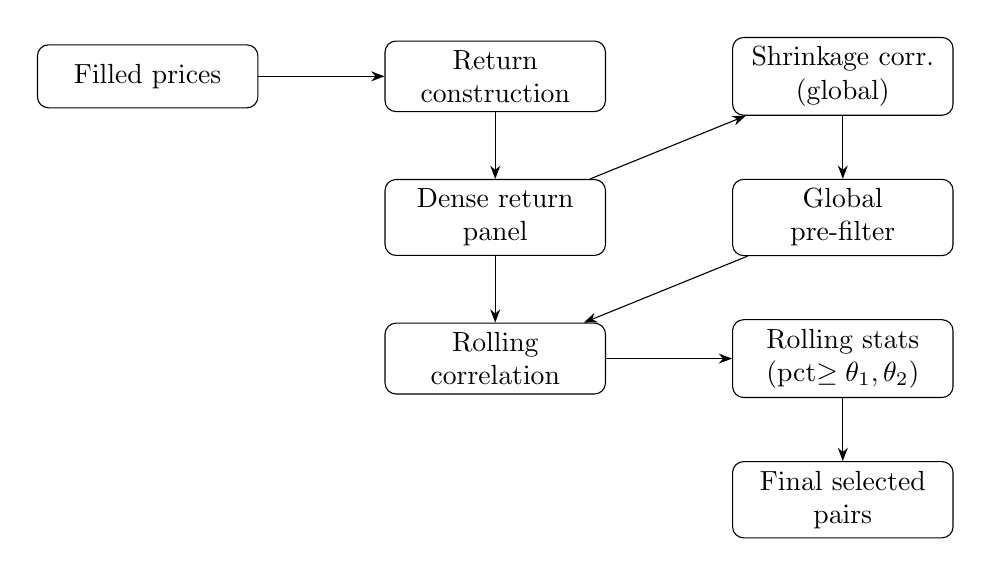
\begin{tikzpicture}[
    >=Stealth,
    node distance=10mm and 14mm,
    block/.style={
      draw,
      rectangle,
      rounded corners,
      align=center,
      minimum width=28mm,
      minimum height=8mm
    },
    every edge/.style={draw,->}
  ]
  \matrix (m) [row sep=8mm, column sep=16mm] {
    \node[block] (filled) {Filled prices}; &
    \node[block] (retclean) {Return\\construction}; &
    \node[block] (shrink) {Shrinkage corr.\\(global)}; \\
    &
    \node[block] (dense) {Dense return\\panel}; &
    \node[block] (prefilter) {Global\\pre-filter}; \\
    &
    \node[block] (rollcorr) {Rolling\\correlation}; &
    \node[block] (rollstats) {Rolling stats\\(pct$\ge \theta_1,\theta_2$)}; \\
    &
    &
    \node[block] (final) {Final selected\\pairs}; \\
  };
  \path (filled) edge (retclean)
        (retclean) edge (dense)
        (dense) edge (shrink);
  \path (shrink) edge (prefilter)
        (dense) edge (rollcorr)
        (prefilter) edge (rollcorr)
        (rollcorr) edge (rollstats)
        (rollstats) edge (final);
  \end{tikzpicture}
  \caption{Schematic overview of the correlation-screening procedure, from filled prices to the final set of selected trading pairs.}
  \label{fig:corr-pipeline}
\end{figure}
\subsubsection{Return Construction}

Given the cleaned and filled execution close-price panel
\(P^{\mathrm{exec}}_{t,i}\) described above, we work with one-period log returns
\[
  r_{t,i} \;=\; \log P^{\mathrm{exec}}_{t,i} - \log P^{\mathrm{exec}}_{t^{-},i},
\]
where \(t\) indexes NYSE trading days on the aligned calendar and \(i\) indexes
symbols. Here, whenever \(t\) is not the first element of
\(\mathcal{T}^{\mathrm{pair}}\), the symbol \(t^{-}\) denotes the immediately
preceding NYSE trading day in \(\mathcal{T}^{\mathrm{pair}}\).

We first construct the log-return matrix
\[
  R = (r_{t,i})
\]
by taking first differences of the logarithms along the time axis. Define the
raw return-index set
\[
  \mathcal{T}^{\mathrm{ret}}
  \;:=\;
  \mathcal{T}^{\mathrm{pair}}\setminus\{\min \mathcal{T}^{\mathrm{pair}}\}.
\]
The first trading day in \(\mathcal{T}^{\mathrm{pair}}\) is excluded because no
prior price within \(\mathcal{T}^{\mathrm{pair}}\) is available for that date.

In the baseline specification, the second trading date is removed
globally during return-panel preparation, due to a leading gap, while no symbols are dropped.
Denoting this excluded date by \(t^\dagger \in \mathcal{T}^{\mathrm{ret}}\), we define the cleaned return-index set by
\[
  \widetilde{\mathcal{T}}^{\mathrm{ret}}
  \;:=\;
  \mathcal{T}^{\mathrm{ret}} \setminus \{t^\dagger\}.
\]
The resulting cleaned return panel is therefore
\[
  \widetilde R
  \;=\;
  (r_{t,i})_{t\in \widetilde{\mathcal{T}}^{\mathrm{ret}},\, i\in\mathcal I},
\]
which is dense on \(\widetilde{\mathcal{T}}^{\mathrm{ret}} \times \mathcal I\).

\subsubsection{Shrinkage Covariance and Correlation}

Based on the dense cleaned return panel \(\widetilde R\), we estimate a
covariance matrix of asset returns \(\Sigma\) using the Ledoit--Wolf shrinkage
estimator \cite{ledoit2004well}. This estimator can be viewed as shrinking the
sample covariance matrix towards a multiple of the identity with a data-driven
shrinkage intensity, which improves conditioning and reduces estimation noise in
settings with many assets and a finite sample of returns.

Let
\[
N_{\text{eff}} := |\mathcal I|
\]
denote the size of the effective analysis universe. In the baseline
specification considered here,
\[
N_{\text{eff}} = 2167.
\]

The Ledoit--Wolf estimator is numerically well behaved, but finite-precision
arithmetic can still induce slight asymmetries or near-zero eigenvalues in the
estimated covariance matrix. To guard against such numerical artefacts, we
symmetrise the covariance estimate and, if necessary, apply a small positive
eigenvalue floor\footnote{We use 
an eigenvalue tolerance of $10^{-12}$ to detect ill-conditioning 
and project to positive-definite space with floor $10^{-8}$.} before converting covariance to correlation. This step is a
numerical stabilisation device and, in our setting, has no material effect on
the substantive screening logic.

From the resulting shrinkage covariance matrix we construct a correlation matrix
\(C=(C_{ij})\) in the usual way,
\[
  C_{ij}
  \;=\;
  \frac{\Sigma_{ij}}{\sqrt{\Sigma_{ii}\,\Sigma_{jj}}},
  \qquad i,j=1,\dots,N_{\text{eff}}.
\]
This yields the global correlation matrix used for the initial pair pre-filter.

\subsubsection{Global correlation pre-filter}

From the shrinkage-based correlation matrix \(C = (C_{ij})\) we construct an
initial candidate set of pairs by retaining only entries with
\(C_{ij} \ge \tau_{\text{corr}}\), where \(\tau_{\text{corr}} = 0.80\) in the
baseline specification summarised in Table~\ref{tab:analysis_hyperparams}. We
restrict attention to the upper triangle \(i<j\) and store each pair in a
canonical ``A--B'' form with the lexicographically smaller ticker first.
Self-pairs \((i=j)\) are excluded by construction. This global correlation
screen filters out 99.98\% of all possible symbol pairs in the baseline run
(retaining 529 out of 2{,}346{,}861 pairs) and thereby substantially reduces
the computational load of the subsequent rolling-correlation and persistence
analysis.

\subsubsection{Rolling-Window Correlation}\label{sec:rolling-corr}

All rolling correlation statistics are computed on the cleaned return-index set
\(\widetilde{\mathcal{T}}^{\mathrm{ret}}\) and hence use only information
strictly prior to the backtest start date. Let \(W_{\text{roll}}\) denote the
window length in trading days and \(\Delta\) the step size between consecutive
window starts. In the baseline specification, as summarised in
Table~\ref{tab:analysis_hyperparams}, we set \(W_{\text{roll}} = 84\) and
\(\Delta = 21\); the notation here is kept general. Write the cleaned
return-index set in increasing order as
\[
  \widetilde{\mathcal{T}}^{\mathrm{ret}}
  =
  \{\tilde t_1 < \cdots < \tilde t_{|\widetilde{\mathcal{T}}^{\mathrm{ret}}|}\}.
\]
For each integer \(w \ge 1\) we define a window
\[
  \mathcal{T}^{\mathrm{roll}}_w
  :=
  \{\tilde t_{k_w}, \tilde t_{k_w+1}, \dots, \tilde t_{k_w+W_{\text{roll}}-1}\},
\]
where \(k_1 = 1\) and \(k_{w+1} = k_w + \Delta\). We retain all windows
\(\mathcal{T}^{\mathrm{roll}}_w\) for which
\[
  k_w + W_{\text{roll}} - 1 \le |\widetilde{\mathcal{T}}^{\mathrm{ret}}|.
\]

The rolling correlation estimation is restricted to the subset of symbols that
appear in at least one global candidate pair from the static pre-filter.
Formally, let \(\mathcal{P}\) denote the set of pairs \((i,j)\) with
\(C_{ij} \ge \tau_{\text{corr}}\) in the global correlation screen. In each
window \(\mathcal{T}^{\mathrm{roll}}_w\), we restrict the dense cleaned return panel
\(\widetilde R\) to the rows in \(\mathcal{T}^{\mathrm{roll}}_w\) and to the columns
corresponding to symbols that appear in at least one pair in \(\mathcal{P}\).

For each retained window \(\mathcal{T}^{\mathrm{roll}}_w\), we estimate a shrinkage covariance
matrix \(\Sigma^{(w)}\) on the restricted returns and derive the corresponding
correlation matrix \(C^{(w)} = (C^{(w)}_{ij})\) using the same
shrinkage-based covariance-to-correlation construction as in the static case.
For a candidate pair \(p=(i,j)\in\mathcal{P}\), the rolling correlation in
window \(w\) is then defined by
\[
  \rho_p(w) \;=\; C^{(w)}_{ij}.
\]
Let \(K_{\mathrm{roll}}\) denote the number of retained rolling windows. Under the baseline
specification described above, the cleaned return-index set
\(\widetilde{\mathcal{T}}^{\mathrm{ret}}\), together with
\(W_{\text{roll}}=84\) and \(\Delta=21\), yields \(K_{\mathrm{roll}}=20\) retained rolling
windows.

For two correlation thresholds \(\theta_1 < \theta_2\) we compute the fraction
of windows in which the pair meets or exceeds each threshold,
\[
  \operatorname{pct}_{\theta_\ell}(p)
  \;=\;
  100 \cdot \frac{1}{K_{\mathrm{roll}}}
  \sum_{w=1}^{K_{\mathrm{roll}}} \mathbf{1}\{\rho_p(w) \ge \theta_\ell\},
  \qquad \ell \in \{1,2\}.
\]
Throughout, \(\operatorname{pct}_{\theta}(p)\) is expressed in percent; the
thresholds \(\pi_{1,\min}\) and \(\pi_{2,\min}\) are therefore specified on the
same 0--100 scale. These percentages measure the temporal persistence of high
correlation: \(\operatorname{pct}_{\theta_1}(p)\) reflects how often the pair is
at least moderately correlated, while \(\operatorname{pct}_{\theta_2}(p)\)
emphasises episodes of particularly strong comovement. In the baseline
specification reported in Table~\ref{tab:analysis_hyperparams} we set
\(\theta_1 = 0.75\) and \(\theta_2 = 0.85\); the two-threshold notation is
retained for generality.

\paragraph{Final pair selection rule}

Statistical significance testing is not used in the final screening rule.
Instead, selection is based on persistent high rolling correlation. Specifically,
we impose minimum persistence requirements on the fraction of windows above the
lower and higher correlation thresholds \(\theta_1\) and \(\theta_2\),
respectively,
\[
  \operatorname{pct}_{\theta_1}(p)
  \;\ge\;
  \pi_{1,\min}
  \qquad\text{and}\qquad
  \operatorname{pct}_{\theta_2}(p)
  \;\ge\;
  \pi_{2,\min}.
\]

A candidate pair \(p\) enters the final selected set if and only if both of the
following conditions hold:
\begin{enumerate}[noitemsep]
  \item the lower-threshold persistence criterion
        \(\operatorname{pct}_{\theta_1}(p) \ge \pi_{1,\min}\) holds;
  \item the higher-threshold persistence criterion
        \(\operatorname{pct}_{\theta_2}(p) \ge \pi_{2,\min}\) holds.
\end{enumerate}

\begin{table}[ht]
  \centering
  \caption{Pair-screening pipeline on the training window (baseline specification).}
  \label{tab:pair_screening_pipeline}
  \begin{tabular}{p{0.68\linewidth}rr}
    \toprule
    Stage & \# pairs & \% of previous \\
    \midrule
    All possible pairs in universe (\(N_{\text{eff}} = 2167\))
      & 2{,}346{,}861 & 100.0 \\
    Global correlation filter (\(C_{ij} \ge 0.80\))
      & 529 & 0.02 \\
    Selected pairs (persistence thresholds \(\pi_{1,\min},\pi_{2,\min}\))
      & 109 & 20.6 \\
    \bottomrule
  \end{tabular}
\end{table}

\begin{table}[ht]
  \centering
  \caption{Key analysis hyperparameters and thresholds}
  \label{tab:analysis_hyperparams}
  \begin{tabular}{ll}
    \toprule
    Quantity & Value \\
    \midrule
    Rolling window length \(W_{\text{roll}}\) (days) & 84 \\
    Rolling step size \(\Delta\) (days) & 21 \\
    Global correlation threshold \(\tau_{\text{corr}}\) & 0.80 \\
    Low/high correlation thresholds \((\theta_1, \theta_2)\) & \((0.75,\, 0.85)\) \\
    Minimum persistence (lower threshold) \(\pi_{1,\min}\) & \(60\%\) \\
    Minimum persistence (higher threshold) \(\pi_{2,\min}\) & \(30\%\) \\
    \bottomrule
  \end{tabular}
\end{table}

The hyperparameters in Table~\ref{tab:analysis_hyperparams} are chosen ex ante
as conservative regularisation parameters rather than as the outcome of an
extensive search over configurations. In particular, the global correlation
threshold is set to ensure that only strongly co-moving pairs enter the
screening stage, while the persistence thresholds further restrict the final
selected set to pairs whose high correlation is also temporally persistent. We
deliberately refrain from tuning these hyperparameters to maximise in-sample or
backtest performance, in line with broader warnings about data mining and
backtest overfitting in empirical asset-pricing research
\cite{harvey2016and,bailey2017probability}.

\paragraph{Interpretation and limitations of the screening stage}

The procedures described above are designed as a pragmatic statistical screening
layer rather than as a fully rigorous inferential test. The combination of a
global correlation filter and rolling-window diagnostics offers a
computationally tractable way of focusing attention on pairs with persistent
high comovement, while downweighting spurious relationships that arise from
sampling noise in a high-dimensional universe.

At the same time, several caveats are important for interpretation:

\begin{itemize}[noitemsep]
  \item \textbf{Screening rather than formal inference.}
        The correlation-based screening stage is intended as a conservative
        dimensionality-reduction and prioritisation device, not as a formal
         procedure with exact frequentist error guarantees.
        The reported thresholds should therefore be interpreted as pragmatic
        selection rules rather than as the output of fully rigorous statistical
        inference.

  \item \textbf{Common-factor comovement.}
        The screening stage operates on execution close series without
        explicitly removing common market or sector factors. As a result, part
        of the measured correlation may reflect shared factor exposures rather
        than pair-specific linkages \cite{fama1993common}.

  \item \textbf{Thresholds and hyperparameter sensitivity.}
        The correlation thresholds \((\theta_1,\theta_2)\) and the minimum
        persistence levels \((\pi_{1,\min}, \pi_{2,\min})\) are pre-specified
        hyperparameters. While the specification used in our experiments is
        conservative and fixed ex ante, any aggressive tuning of these
        thresholds to maximise backtest performance would introduce an
        additional layer of selection bias
        \cite{harvey2016and,bailey2017probability}.

  \item \textbf{Correlation vs.\ tradable mean reversion.}
        The screening stage is intended as a robust preliminary filter for
        constructing a plausible pair universe, rather than as a definitive test
        of tradable mean-reversion structure. It operates solely on return
        correlations and therefore does not by itself establish a stable
        equilibrium relationship between the two assets. Cointegration is not
        used at this screening stage; instead, it is imposed later as a
        split-level \emph{tradability check} (Engle--Granger) within each
        walk-forward training block (see Section~\ref{sec:per_split_loader}).
        A pair that passes the correlation-based filters should therefore be
        interpreted only as a candidate for further investigation. The
        subsequent cointegration check, spread construction and backtest stages
        provide the main statistical and economic validation of tradable
        mean-reversion behaviour.
\end{itemize}


\section{Baseline Mean-Reversion Strategy}

We now formalize the benchmark trading rule used throughout the study.
Conditional on a given tradable pair \(p=(i,j)\) and a given walk-forward
evaluation block, the upstream calibration step, discussed later, delivers all pair-specific
inputs required by the strategy. In particular, we take as fixed for the
current pair and evaluation block a hedge coefficient
\(\beta \in \mathbb R \setminus \{0\}\), a rolling normalization window
\(W \in \mathbb N\), a minimum effective lookback
\(m \in \mathbb N\) satisfying \(1 \le m \le W\), thresholds satisfying
\[
  0 < z_{\mathrm{exit}} < z_{\mathrm{ent}} < z_{\mathrm{stop}},
\]
a maximum holding horizon \(H_{\max} \in \mathbb N\), a cooldown length
\(C_{\mathrm{cool}} \in \mathbb N_0\), and the risk-control constants introduced below.
Throughout this section, all such quantities are treated as exogenous inputs to
the baseline rule for the given pair and split.

Let \(\mathcal T^{(p)}\) denote the ordered set of trading dates relevant for the
current pair, and write
\[
  Y_t := P^{\mathrm{exec}}_{t,i},
  \qquad
  X_t := P^{\mathrm{exec}}_{t,j},
  \qquad t \in \mathcal T^{(p)},
\]
for the execution-relevant prices of the two assets. Within the current
out-of-sample block, we distinguish between an \emph{entry-eligible} date set
\(\mathcal T^{\mathrm{ent}} \subseteq \mathcal T^{(p)}\) and a possibly larger
\emph{evaluation} set \(\mathcal T^{\mathrm{eval}} \subseteq \mathcal T^{(p)}\) such
that
\[
  \mathcal T^{\mathrm{ent}} \subseteq \mathcal T^{\mathrm{eval}} \subseteq \mathcal T^{(p)}.
\]
New positions may be initiated only on dates in
\(\mathcal T^{\mathrm{ent}}\), whereas already open positions may continue to
be managed and liquidated on all dates in \(\mathcal T^{\mathrm{eval}}\).
Thus \(\mathcal T^{\mathrm{ent}}\) defines the entry window, while
\(\mathcal T^{\mathrm{eval}}\) defines the full signal-management window. A
signal generated on a date in \(\mathcal T^{\mathrm{ent}}\) is executed with
the strategy's one-bar lag only if the corresponding execution date still lies
in \(\mathcal T^{\mathrm{eval}}\); otherwise the signal is not implemented as an executed trade. If a
position remains open through the end of \(\mathcal T^{\mathrm{eval}}\), it is
liquidated at the last available execution date in
\(\mathcal T^{\mathrm{eval}}\) as a terminal boundary convention. Outside
\(\mathcal T^{\mathrm{eval}}\), the strategy is flat by convention. At the
beginning of each evaluation block, the active-position state is reset to flat,
and no pending entry or liquidation instruction is carried into the block.

\subsection{Spread Representation and Causal Rolling Standardization}

The baseline strategy assumes that relative mispricing is summarized by the
one-dimensional spread
\[
  S_t \;=\; Y_t - \beta X_t.
\]
The scalar \(\beta\) defines the linear hedge that maps the two asset prices
into a signed spread. For \(\beta>0\), this coincides with the usual long-short
residual interpretation. For \(\beta<0\), the same algebraic representation
remains well defined, but it should be interpreted simply as a signed linear
combination of the two legs rather than as a universal rich-versus-cheap
statement. The baseline trading rule depends only on the sign and standardized
magnitude of \(S_t\), not on any stronger restriction on the sign of
\(\beta\).

To make spread deviations comparable over time, the strategy standardizes the
current spread by a trailing window of \emph{strictly past} spread
observations. For each \(t \in \mathcal T^{\mathrm{eval}}\), let
\(\mathcal W_t \subseteq \mathcal T^{(p)}\) denote the right-aligned lookback set
containing up to the \(W\) most recent dates strictly before \(t\) for which
admissible spread observations are available to the strategy at time \(t\).
Here an admissible spread observation means a date in the history made
available to the rolling procedure at time \(t\) for which both
execution-relevant leg prices are observed, so that \(S_u\) can be formed.
Thus, at the beginning of the evaluation block, \(\mathcal W_t\) may be seeded
by the most recent admissible pre-evaluation observations from the
corresponding training side of the split; as the backtest advances through the
evaluation block, these are causally replaced by newly realized
evaluation-period observations in the same rolling-window construction. Hence
no future observation enters the signal at date \(t\), and no observation older
than the \(W\) most recent admissible past dates can enter \(\mathcal W_t\).

Whenever \(|\mathcal W_t| \ge m\), the rolling location and scale estimators
are
\[
  \mu_t
  \;:=\;
  \frac{1}{|\mathcal W_t|}
  \sum_{u \in \mathcal W_t} S_u,
  \qquad
  \sigma_t
  \;:=\;
  \left(
    \frac{1}{|\mathcal W_t|}
    \sum_{u \in \mathcal W_t} (S_u-\mu_t)^2
  \right)^{1/2},
\]
and, whenever additionally \(\sigma_t>0\), the corresponding rolling Z-score is
\[
  Z_t \;:=\; \frac{S_t-\mu_t}{\sigma_t}.
\]
Thus the scale estimate uses the population convention on the trailing window.
If fewer than \(m\) admissible past spread observations are available, or if
\(\sigma_t=0\), then \(Z_t\) is treated as undefined.

This construction yields a dimensionless measure of the current spread
dislocation relative to its recent local history. Large values of \(|Z_t|\)
indicate that the spread is far from its recent rolling center in units of its
recent rolling scale. The baseline strategy interprets such events as potential
mean-reversion opportunities.

\subsection{Signal State, Entry Logic, Exit Logic, and Cooldown}

Let \(D_t \in \{-1,0,1\}\) denote the directional state of the currently active
position at the start of signal evaluation on date
\(t \in \mathcal T^{\mathrm{eval}}\), after any instructions scheduled for
execution on date \(t\) have been processed, where
\[
  D_t =
  \begin{cases}
    1, & \text{long spread},\\
    0, & \text{flat},\\
    -1, & \text{short spread}.
  \end{cases}
\]
These labels refer to the sign of spread exposure. The corresponding executed
leg directions are defined later through the trade-mapping equations and depend
on both \(D_t\) and the sign of \(\beta\). Signals generated on date \(t\) do
not change \(D_t\) immediately; rather, they create pending entry or
liquidation instructions for the next available execution date.
A position opened by an entry instruction executed on date \(t\) is recorded as active from \(t\) onward, but it is not subjected to liquidation testing again on \(t\); liquidation logic is first applied on the next subsequent date in \(\mathcal T^{\mathrm{eval}}\) on which the position is still active at the start of signal evaluation.

For notational economy, whenever \(t\) is not the first element of
\(\mathcal T^{\mathrm{eval}}\), write \(t^{-}\) for the immediately preceding
trading date in \(\mathcal T^{\mathrm{eval}}\). For the first element of
\(\mathcal T^{\mathrm{eval}}\), \(Z_{t^-}\) is treated as undefined by
convention; consequently, any comparison involving \(Z_{t^-}\) is taken to be
false, whereas the statement ``\(Z_{t^-}\) is undefined'' is taken to hold.
The baseline rule is a crossing-based strategy. Entries are evaluated only on
dates in \(\mathcal T^{\mathrm{ent}}\) that begin in the flat state and are
not blocked by the cooldown rule described below. In particular, if a position
is already open at the start of signal evaluation on date \(t\), then only the
exit logic is evaluated on that date; no same-date reversal is permitted.

A long-spread entry signal is generated on date \(t \in \mathcal T^{\mathrm{ent}}\)
if and only if
\[
  Z_t \text{ is defined},
  \qquad
  -z_{\mathrm{stop}} < Z_t \le -z_{\mathrm{ent}},
\]
and either
\[
  Z_{t^-} \text{ is undefined}
  \qquad\text{or}\qquad
  Z_{t^-} > -z_{\mathrm{ent}}.
\]
A short-spread entry signal is generated on date
\(t \in \mathcal T^{\mathrm{ent}}\) if and only if
\[
  Z_t \text{ is defined},
  \qquad
  z_{\mathrm{ent}} \le Z_t < z_{\mathrm{stop}},
\]
and either
\[
  Z_{t^-} \text{ is undefined}
  \qquad\text{or}\qquad
  Z_{t^-} < z_{\mathrm{ent}}.
\]
Hence entries require a \emph{new crossing} into the admissible entry band
\[
  z_{\mathrm{ent}} \le |Z_t| < z_{\mathrm{stop}},
\]
rather than mere persistence beyond an already-crossed threshold. This avoids
repeated re-entry while the Z-score remains in the same extreme region and
excludes immediate entry into the stop region by construction. At the first
date of \(\mathcal T^{\mathrm{eval}}\), however, the convention
\(Z_{t^-}\) undefined implies that an admissible in-band observation may
trigger entry even without a within-block threshold crossing; this is the
block-initialization convention induced by resetting the active-position state
to flat at the start of each evaluation block. Likewise, after a stop-out or
any other exit, re-entry still requires a fresh admissible crossing condition;
a mere return from the stop region into the entry band does not by itself
generate a new entry signal.

Once a position has become active, it remains active until the first date on
which at least one exit condition is met. Let \(a_t\) denote the age of the
currently active position on date
\(t \in \mathcal T^{\mathrm{eval}}\), measured in signal-evaluation days rather
than execution days. If an admissible entry signal is generated on date
\(s \in \mathcal T^{\mathrm{ent}}\) and is successfully executed on the next
available execution date \(\tau>s\), then the directional state becomes
\(D_\tau \in \{-1,1\}\), and the age is initialized at \(a_\tau=0\). On each
subsequent date in \(\mathcal T^{\mathrm{eval}}\) that begins with the position
still active, the age is incremented by one. Thus \(H_{\max}\) limits the
signal-evaluation holding duration; under the one-bar execution lag, the
realized execution-to-liquidation duration may differ accordingly. Whenever a
position is open at the start of signal evaluation on date \(t\), a
liquidation signal is generated if at least one of the following conditions
holds:
\[
  Z_t \text{ is undefined},
  \qquad
  |Z_t| \le z_{\mathrm{exit}},
  \qquad
  |Z_t| \ge z_{\mathrm{stop}},
  \qquad
  a_t \ge H_{\max},
\]
or if the spread has traversed the entire signal range into the opposite entry
region without entering the stop region, that is,
\[
  D_t=1 \ \text{and}\ z_{\mathrm{ent}} \le Z_t < z_{\mathrm{stop}},
  \qquad \text{or} \qquad
  D_t=-1 \ \text{and}\ -z_{\mathrm{stop}} < Z_t \le -z_{\mathrm{ent}}.
\]
The first condition is an operational liquidation rule for signal
unavailability, the second corresponds to reversion into the neutral band, the
third is a stop rule based on entry into the stop region, the fourth is a
finite holding-horizon cap, and the fifth is a symmetry rule that forces
liquidation once the Z-score has moved from one entry extreme all the way into
the opposite entry region without already being classified as a stop-out.

After an executed liquidation, the strategy enters a cooldown state of length
\(C_{\mathrm{cool}}\). The liquidation date itself is not counted among the
blocked future dates. Rather, the next \(C_{\mathrm{cool}}\) dates in
\(\mathcal T^{\mathrm{ent}}\) following the liquidation date are blocked from
initiating a new position, even if the Z-score again crosses an entry
threshold. Since an active position is not eligible for new entry signals and
liquidation instructions are implemented only with the one-bar lag, same-date
reversal is impossible. This cooldown acts as a regularization device against
immediate whipsaw re-entry in oscillatory spread regimes.

\subsection{Execution Mapping and Trade-Level PnL}

The state process \((D_t)\) is an active-position-level object. In the backtest,
signals are implemented with a one-bar execution lag. Accordingly, if an
admissible entry signal is generated on signal date \(s\), it creates a pending
candidate entry for the next available execution date \(\tau>s\). The
corresponding trade is entered only if that candidate passes the execution-side
admissibility and sizing checks at date \(\tau\). Likewise, liquidation signals
generated during the life of the position are implemented at the corresponding
lagged execution date. The only exception is the terminal boundary convention
stated above: if a position remains open through the end of
\(\mathcal T^{\mathrm{eval}}\), it is liquidated on the last available
execution date in that set. The baseline strategy considered here therefore
separates signal formation from trade execution.

Let \(q_\tau \in \mathbb N\) denote the executed integer trade size of a trade
that is actually entered at date \(\tau\). Its construction is determined by
the sizing rule introduced below: a candidate size is first computed, and an
entry is executed only if the resulting admissible integer size is strictly
positive. Let \(d_s \in \{-1,1\}\) denote the direction of the entry signal
generated on signal date \(s\), where \(d_s=1\) for a long-spread signal and
\(d_s=-1\) for a short-spread signal. If the corresponding candidate is
successfully executed at date \(\tau\), the executed leg units at entry are
therefore
\[
  n^Y_\tau = d_s q_\tau,
  \qquad
  n^X_\tau = -d_s \beta q_\tau.
\]
Thus the hedge-leg units are generally real-valued when \(\beta\) is not an
integer. In particular, the signed \(X\)-leg position depends jointly on the
spread direction \(d_s\) and the sign of \(\beta\). For \(\beta>0\), a
long-spread trade is long \(Y\) and short \(X\), while a short-spread trade
reverses these directions. For \(\beta<0\), the two executed legs instead have
the same sign.

If the position entered at \(\tau\) is exited at date \(u>\tau\), then its
pre-cost trade-level PnL is
\[
  \Pi_{\tau,u}
  \;=\;
  n^Y_\tau (Y_u - Y_\tau)
  \;+\;
  n^X_\tau (X_u - X_\tau).
\]
This expression makes explicit that the benchmark is a two-leg spread-based
position whose payoff is generated by the joint price path of the two assets
under the hedge coefficient \(\beta\).

\subsection{Risk-Based Unit Sizing}

Each candidate entry is sized by combining a stop-distance-based risk budget
with separate caps on gross trade notional and, when available, market
participation. Let \(K_0>0\) denote the fixed capital base used for candidate
trade construction in the current backtest run, and let
\(\rho_{\mathrm{risk}} \in (0,1)\) be the fraction of \(K_0\) that may be risked on a single
trade under the stop-loss proxy described below.

Consider an admissible entry signal generated on signal date \(s\), with
execution scheduled for the next available date \(\tau>s\). Define the
remaining Z-distance to the stop at the \emph{signal} date by
\[
  \delta_s
  \;:=\;
  z_{\mathrm{stop}} - |Z_s|.
\]
Because admissible entries satisfy
\(z_{\mathrm{ent}} \le |Z_s| < z_{\mathrm{stop}}\), one has \(\delta_s>0\).
Since
\[
  Z_s = \frac{S_s-\mu_s}{\sigma_s},
\]
one unit of Z-score distance corresponds to \(\sigma_s\) units in spread space.
The per-unit stop-risk proxy is therefore
\[
  r_s \;:=\; \delta_s \sigma_s.
\]
This converts the remaining distance to the stop from standardized units back
into spread-price units using the same rolling scale that defines the signal
itself. It is an ex ante proxy rather than an exact pathwise loss bound,
because both the rolling normalization objects and the realized execution prices
continue to evolve after the signal date. Accordingly, the stop-risk budget is
anchored at the signal date \(s\), whereas the notional-based caps introduced
below are evaluated at the actual execution date \(\tau\).

The unconstrained risk-budget size is
\[
  q^{(0)}_s
  \;:=\;
  \left\lfloor \frac{\rho_{\mathrm{risk}} K_0}{r_s} \right\rfloor.
\]
Next, define the gross per-unit entry notional at the \emph{execution} date by
\[
  g_\tau := |Y_\tau| + |\beta|\,|X_\tau|.
\]
Let \(\eta \in (0,1)\) denote the maximum admissible fraction of \(K_0\) that
may be committed in gross trade notional. The trade-notional cap then yields
\[
  q^{(1)}_\tau
  \;:=\;
  \min\!\left\{
    q^{(0)}_s,
    \left\lfloor \frac{\eta K_0}{g_\tau} \right\rfloor
  \right\}.
\]

Finally, when a valid pair-level liquidity proxy is available, the strategy
imposes an additional participation cap. Let \(A_p>0\) denote the pair-level
ex ante dollar-liquidity proxy used by the implementation for pair \(p\); under
the present implementation, \(A_p\) is fixed across candidate entries for the
pair within the current evaluation block whenever such a proxy is available.
Let \(\kappa \in (0,1)\) be the maximum participation fraction. The final
candidate trade size is then
\[
  q_\tau^{\mathrm{cand}}
  \;:=\;
  \min\!\left\{
    q^{(1)}_\tau,
    \left\lfloor \frac{\kappa A_p}{g_\tau} \right\rfloor
  \right\}.
\]
If no valid liquidity proxy is available, the participation constraint is not
applied and the final candidate size is simply
\[
  q_\tau^{\mathrm{cand}} := q^{(1)}_\tau.
\]

Hence candidate trade construction combines three distinct controls: a
signal-date stop-risk budget, an execution-date gross-notional cap, and, when
available, a pair-level participation cap. If any required quantity is
undefined, or if the resulting final candidate size satisfies
\[
  q_\tau^{\mathrm{cand}} \le 0,
\]
the candidate entry is discarded and no trade is opened. Otherwise, the entry
is accepted and the executed trade size is
\[
  q_\tau := q_\tau^{\mathrm{cand}} \in \mathbb N.
\]

\subsection{Interpretation}

The benchmark strategy is therefore a causal threshold mean-reversion rule on a
linearly hedged spread. Its statistical core is the view that sufficiently
large standardized spread deviations are locally transitory: when the spread
moves far enough from its recent rolling center, but not yet into the stop
region, the strategy takes a two-leg position betting on partial reversion
toward the neutral band. Its risk-control core is equally important. Exposure
is not chosen as an arbitrary fixed number of shares, but is obtained from an
ex ante mapping from stop distance and capital into permissible trade units,
followed by notional and liquidity caps.

Taken together, these elements yield a parsimonious benchmark architecture:
\begin{enumerate}[leftmargin=*, itemsep=2pt, topsep=2pt]
  \item represent relative mispricing by the linear spread \(S_t\),
  \item normalize the spread into a strictly past-only rolling Z-score \(Z_t\),
  \item enter only on new crossings into the admissible entry band while flat
        and outside cooldown,
  \item exit on signal unavailability, reversion, stop-out, holding-horizon
        exhaustion, or full traversal into the opposite entry region,
  \item map lagged signals into executed two-leg trades and size candidate
        entries through stop-risk, notional, and optional participation
        constraints.
\end{enumerate}
This benchmark serves as the theoretical foundation for the filtered variant
introduced subsequently.

\section{Markov Entry Overlay}

The filtered variant augments the baseline rule by an additional
\emph{entry-admissibility} screen based on a finite-state Markov approximation
to the dynamics of the rolling Z-score process. The overlay does not redefine
the spread, the rolling standardization, the exit logic, or the sizing rule.
Its role is only to screen baseline entry \emph{signals} on their signal date:
a baseline crossing may generate a candidate entry signal only if the Markov
gate also permits it. The subsequent one-bar execution lag and the later
intent-level checks of the baseline runtime remain unchanged.

For the current pair and walk-forward split, fix overlay parameters
\[
  L \in \mathbb N,
  \qquad
  \pi_{\min} \in [0,1],
  \qquad
  n_{\mathrm{train}}^{\min} \in \mathbb N,
  \qquad
  n_{\mathrm{state}}^{\min} \in \mathbb N,
  \qquad
  \lambda \in \mathbb R_{\ge 0},
\]
together with state thresholds
\[
  0 \le z_{\mathrm{neu}}^{\mathrm{MC}} < z_{\mathrm{ent}}^{\mathrm{MC}}.
\]
Here \(L\) is the forecasting horizon in trading days,
\(\pi_{\min}\) is the minimum required reversion probability,
\(n_{\mathrm{train}}^{\min}\) is the minimum number of defined training-state
observations required to activate the overlay,
\(n_{\mathrm{state}}^{\min}\) is the minimum support required for a specific
current state to be screened rather than passed through, and \(\lambda\) is an
optional transition-smoothing constant. Under the present implementation,
\(z_{\mathrm{neu}}^{\mathrm{MC}}\) is typically taken equal to
\(z_{\mathrm{exit}}\) and \(z_{\mathrm{ent}}^{\mathrm{MC}}\) equal to
\(z_{\mathrm{ent}}\), unless explicitly overridden by configuration.

The overlay is fitted once on the training-side history of the current
walk-forward split and then held fixed throughout the subsequent
out-of-sample block; it does not update its transition estimates online during
evaluation. Let
\[
  \mathcal T^{\mathrm{MC,tr}} = \{t_1 < t_2 < \dots < t_M\}
  \subseteq \mathcal T^{(p)}
\]
denote the ordered set of training-history dates used for Markov fitting.

For any date \(t\) on which the baseline rolling Z-score \(Z_t\) is available,
define the discretized state \(R_t\) by
\[
  R_t
  :=
  \begin{cases}
    0, & \text{if } Z_t \text{ is defined and } Z_t \le -z_{\mathrm{ent}}^{\mathrm{MC}},\\
    1, & \text{if } Z_t \text{ is defined and } -z_{\mathrm{ent}}^{\mathrm{MC}} < Z_t < -z_{\mathrm{neu}}^{\mathrm{MC}},\\
    2, & \text{if } Z_t \text{ is defined and } |Z_t| \le z_{\mathrm{neu}}^{\mathrm{MC}},\\
    3, & \text{if } Z_t \text{ is defined and } z_{\mathrm{neu}}^{\mathrm{MC}} < Z_t < z_{\mathrm{ent}}^{\mathrm{MC}},\\
    4, & \text{if } Z_t \text{ is defined and } Z_t \ge z_{\mathrm{ent}}^{\mathrm{MC}},\\
    \text{undefined}, & \text{if } Z_t \text{ is undefined}.
  \end{cases}
\]
These states correspond to extreme negative, inner negative, neutral, inner
positive, and extreme positive Z-score regimes. The overlay is therefore built
on a coarse discretization of the same causal rolling Z-score series already
used by the baseline strategy; no separate Markov-specific Z-score series is
constructed. Under this five-state specification, the outer states \(0\) and
\(4\) pool all observations with
\(|Z_t| \ge z_{\mathrm{ent}}^{\mathrm{MC}}\), including observations that may
also lie in the baseline stop region when
\(z_{\mathrm{stop}} > z_{\mathrm{ent}}^{\mathrm{MC}}\).

Let
\[
  V_a
  :=
  \sum_{\ell=1}^{M}
  \mathbf 1\{R_{t_\ell}=a\},
  \qquad a \in \{0,1,2,3,4\},
\]
denote the training-state visit counts. If
\[
  \sum_{a=0}^4 V_a < n_{\mathrm{train}}^{\min},
\]
the overlay is treated as globally inactive for the current pair and split, and
all baseline entry signals are passed through unfiltered.

Otherwise, transition counts are formed only from directly adjacent
training-history dates for which both states are defined:
\[
  N_{ab}
  :=
  \sum_{\ell=1}^{M-1}
  \mathbf 1\{R_{t_\ell}=a,\ R_{t_{\ell+1}}=b\},
  \qquad a,b \in \{0,1,2,3,4\},
\]
with row sums
\[
  N_a^{\mathrm{out}}
  :=
  \sum_{b=0}^4 N_{ab}.
\]
Thus undefined states are neither removed in advance nor bridged across:
they simply contribute no transition count whenever one side of an adjacent
training pair is undefined. Whenever \(N_a^{\mathrm{out}}>0\), the one-step
transition row is estimated by
\[
  \widehat P^{\mathrm{MC}}_{ab}
  :=
  \frac{N_{ab}+\lambda}{N_a^{\mathrm{out}}+5\lambda},
  \qquad b \in \{0,1,2,3,4\}.
\]
If \(N_a^{\mathrm{out}}=0\), no supported transition row is estimated for state
\(a\); in particular, the implementation does not create an artificial uniform
row from the smoothing constant alone.

To obtain a finite-horizon reversion criterion, the overlay treats the neutral
state \(2\) as absorbing. In addition, unsupported non-neutral rows are treated
as self-absorbing for the horizon calculation only. Formally, define
\(\widetilde P^{\mathrm{MC}}\) by
\[
  \widetilde P^{\mathrm{MC}}_{2b}
  :=
  \mathbf 1\{b=2\},
\]
and, for \(a \neq 2\),
\[
  \widetilde P^{\mathrm{MC}}_{ab}
  :=
  \begin{cases}
    \widehat P^{\mathrm{MC}}_{ab},
    & \text{if } N_a^{\mathrm{out}} > 0,\\[4pt]
    \mathbf 1\{a=b\},
    & \text{if } N_a^{\mathrm{out}} = 0.
  \end{cases}
\]
The finite-horizon neutral-hit probability from state \(a\) is then
\[
  \widehat \pi_L(a)
  :=
  \bigl[(\widetilde P^{\mathrm{MC}})^L\bigr]_{a,2},
  \qquad a \in \{0,1,2,3,4\}.
\]
Because the neutral state is made absorbing, this is the model-implied
probability that the discretized Z-score process reaches the neutral region
within \(L\) trading days.

The fitted probabilities are mapped into an out-of-sample entry gate on the
\emph{signal date}. For a date \(t\) in the evaluation block, let \(a=R_t\)
whenever \(R_t\) is defined. If the overlay is globally active,
\(V_a \ge n_{\mathrm{state}}^{\min}\), and \(N_a^{\mathrm{out}}>0\), define
\[
  G_t
  :=
  \mathbf 1\{\widehat \pi_L(a) \ge \pi_{\min}\}.
\]
If \(R_t\) is undefined, or if any of these support conditions fail, the
implementation uses a pass-through convention and sets \(G_t=1\). Hence weak or
missing support does not create automatic rejection; it merely suppresses the
filter and leaves the baseline entry signal unchanged.

The interaction with the baseline rule is therefore one-sided. On a signal date
\(t\), a baseline crossing contributes a candidate entry signal only if the
corresponding Markov gate also satisfies \(G_t=1\). The later baseline runtime
logic---including flat-state enforcement, cooldown checks, and the one-bar
mapping from signal date to execution date---is applied unchanged downstream.
Accordingly, the Markov condition is necessary for a filtered candidate entry
signal but not by itself sufficient for an executed trade.

No other part of the strategy is altered. In particular, the overlay does not
modify the spread \(S_t\), the rolling standardization
\((\mu_t,\sigma_t,Z_t)\), the exit conditions, the cooldown mechanism, the
execution lag, or the risk-based sizing rule. It is purely a conservative entry
filter that retains only those baseline candidate signals for which the current
discretized Z-score state exhibits sufficiently high training-implied odds of
returning to the neutral band within the prescribed horizon.


\section{Portfolio-Level Risk Management}

The pair-level strategy determines candidate trades, their entry and exit dates,
executed leg units, and trade-level PnL. These candidates are then passed
through a \emph{portfolio-level} risk manager, which does not modify signal
formation or trade sizing, but filters already-constructed trades for portfolio
admissibility.

Let \(\mathcal T^{\mathrm{port}} \subseteq \mathcal T\) denote the ordered set
of dates in the local portfolio-evaluation window, with
\[
  t_0^{\mathrm{port}} := \min \mathcal T^{\mathrm{port}}.
\]
For each candidate trade \(c\), let \(s_c \in \mathcal T^{\mathrm{port}}\) be
its entry date, \(u_c \ge s_c\) its exit date, and \(p_c=(i_c,j_c)\) its traded
pair. Let
\[
  (\nu_c^Y,\nu_c^X)\in\mathbb R^2
\]
denote the signed entry notionals of the two executed legs, where positive
values correspond to long legs and negative values to short legs, and where the
\(Y\)-leg corresponds to symbol \(i_c\) and the \(X\)-leg to symbol \(j_c\).
Define
\[
  g_c^{\mathrm{port}} := |\nu_c^Y| + |\nu_c^X|.
\]
These notionals are portfolio-accounting quantities and are distinct from the
executed leg units \((n_\tau^Y,n_\tau^X)\).

For each candidate trade \(c\), let \(\mathcal O_c\) denote the current set of
previously accepted trades that are still open immediately before candidate
\(c\) is evaluated. Positions entered before \(t_0^{\mathrm{port}}\) and still
live at \(t_0^{\mathrm{port}}\) are included in the initial open book.

Let \(K_c^{\mathrm{port}}\) denote the portfolio capital measure used by the
risk manager immediately before candidate \(c\) is evaluated. Before
evaluation, trades with exit date weakly earlier than \(s_c\) are removed from
\(\mathcal O_c\), realized PnL is credited only once its settlement date is
weakly earlier than \(s_c\) (one-bar lag in the baseline configuration), and
remaining open positions are marked to market at date \(s_c\). Thus all
portfolio caps are evaluated against the contemporaneous portfolio capital
measure \(K_c^{\mathrm{port}}\) just defined.

A candidate trade \(c\) is admitted only if all active portfolio constraints are
satisfied. In the baseline configuration, these are:
\begin{enumerate}[leftmargin=*, itemsep=2pt, topsep=2pt]
  \item at most \(10\) simultaneously open positions;
  \item
  \[
    g_c^{\mathrm{port}} \le 0.30\,K_c^{\mathrm{port}};
  \]
  \item
  \[
    \sum_{h\in\mathcal O_c}\bigl(|\nu_h^Y|+|\nu_h^X|\bigr)
    + g_c^{\mathrm{port}}
    \le 2.5\,K_c^{\mathrm{port}};
  \]
  \item
  \[
    \left|
      \sum_{h\in\mathcal O_c}(\nu_h^Y+\nu_h^X)
      + \nu_c^Y + \nu_c^X
    \right|
    \le 0.30\,K_c^{\mathrm{port}};
  \]
  \item a per-symbol concentration cap.
\end{enumerate}

For each symbol \(a \in \mathcal I\), define the open gross exposure
\[
  E_c(a)
  :=
  \sum_{h\in\mathcal O_c}
  \left(
    |\nu_h^Y|\,\mathbf 1\{i_h=a\}
    +
    |\nu_h^X|\,\mathbf 1\{j_h=a\}
  \right).
\]
Then \(c\) is admissible only if
\[
  E_c(i_c)+|\nu_c^Y| \le 0.35\,K_c^{\mathrm{port}}
  \qquad\text{and}\qquad
  E_c(j_c)+|\nu_c^X| \le 0.35\,K_c^{\mathrm{port}}.
\]
In addition, no symbol may appear in more than two simultaneously open accepted
positions.

Before these cap checks, the implementation applies a heuristic
short-availability screen to short legs only. Under the baseline configuration,
a short leg is rejected if its entry price is below \(5\) USD or its associated
symbol-level ADV proxy is below \(2{,}000{,}000\) USD. If blocking on missing
inputs is enabled, missing required price or ADV information also causes
rejection; if the necessary inputs are unavailable for the run as a whole, the
heuristic is suppressed globally.

Accepted candidates are inserted into the live open-position ledger
immediately, so later candidates on the same date are evaluated sequentially
against the updated portfolio state. Rejected candidates do not enter the
realized strategy path.

The portfolio-level risk manager is therefore a post-construction admissibility
layer that leaves the pair-level signal logic, spread construction, Markov entry
overlay, execution lag, and trade-level sizing rule unchanged.


\section{Walk-Forward Design, Per-Split Pair Filtering, and Hyperparameter Selection}
\label{sec:per_split_loader}

We now describe the walk-forward evaluation path used by the live backtest
pipeline under the baseline configuration considered in this study. The purpose
of this layer is threefold. First, it maps the globally selected pair universe
from the analysis stage into a sequence of rolling train--test splits.
Second, within each split, it applies a train-window-specific tradability screen
and derives pair-level runtime parameters. Third, it optionally selects the
signal thresholds by Bayesian optimization on the training side of the same
walk-forward window before the final out-of-sample run is executed.

Under the active branch studied here, the backtest does not rebuild the full
symbol universe from scratch. Instead, it loads the processed execution panel,
the analysis-stage pair list, and the symbol-level ADV objects from the
upstream analysis artifacts. Let
\[
  \mathcal T^{\mathrm{bt}} \subseteq \mathcal T
\]
denote the ordered runtime calendar on which the walk-forward backtest is
carried out. Unless an explicit backtest range is imposed, the start of
\(\mathcal T^{\mathrm{bt}}\) is the first available trading day on or after the
configured global analysis cutoff, and the end of \(\mathcal T^{\mathrm{bt}}\)
is the last session available in the processed data panel. Nominal month-based
train and test boundaries are mapped to the nearest admissible sessions on this
calendar in a causal and deterministic way: train starts are mapped forward to
the next available session, whereas train and test ends are mapped backward to
the most recent available session.

The walk-forward schedule uses rolling training windows. Accordingly, the
runtime calendar \(\mathcal T^{\mathrm{bt}}\) is partitioned into an ordered
sequence of windows
\[
  \bigl(\mathcal T_b^{\mathrm{tr}}, \mathcal T_b^{\mathrm{te}}\bigr),
  \qquad b=1,\dots,B_{\mathrm{WF}},
\]
where each \(\mathcal T_b^{\mathrm{tr}}\) is a contiguous training block and
each \(\mathcal T_b^{\mathrm{te}}\) is the immediately subsequent contiguous
test block. The windows are generated chronologically from the configured
initial training length, test length, and step size, and any candidate window
that cannot be mapped to valid calendar endpoints is discarded. The resulting
test blocks are required to be non-overlapping after calendar mapping. Let
\[
  t_{\mathrm{start}}^{\mathrm{OOS}} := \min \mathcal T_1^{\mathrm{te}},
  \qquad
  t_{\mathrm{end}}^{\mathrm{OOS}} := \max \mathcal T_{B_{\mathrm{WF}}}^{\mathrm{te}}
\]
denote the global out-of-sample horizon covered by the walk-forward run.

For each walk-forward window \(b\), the pipeline constructs a local backtest
configuration by setting the train split equal to
\(\mathcal T_b^{\mathrm{tr}}\) and the local entry test interval equal to
\(\mathcal T_b^{\mathrm{te}}\). However, positions opened from signals
generated in window \(b\) are not forcibly liquidated at
\(\max \mathcal T_b^{\mathrm{te}}\). Rather, the implementation allows such
positions to continue to be managed and exited on later dates up to
\(t_{\mathrm{end}}^{\mathrm{OOS}}\), consistent with the distinction between the
entry-eligible set \(\mathcal T^{\mathrm{ent}}\) and the broader evaluation set
\(\mathcal T^{\mathrm{eval}}\) used by the strategy itself. This design permits
local entry generation on a rolling schedule while preserving economically
meaningful exit handling for positions that survive beyond the end of a single
window's entry block.

Before any Bayesian optimization is performed, the code prepares the pair data
for the current window. This ordering is important. Bayesian optimization is
therefore always carried out on the same train-window-filtered pair universe
that is subsequently used in the final local backtest; it does not search over,
or rebuild, a different pair set after the optimization stage has finished.

Consider a pair \(p=(i,j)\) carried forward from the upstream analysis stage.
For the current walk-forward window \(b\), let \(Y_t\) and \(X_t\) denote the
execution-close series of the two assets, restricted first to the local
training dates \(\mathcal T_b^{\mathrm{tr}}\) for the purpose of per-split
diagnostics. In the active branch, pair prefiltering is enabled. The two series
are aligned on the common finite observations inside
\(\mathcal T_b^{\mathrm{tr}}\); if the resulting overlap is invalid or contains
fewer than the configured minimum number of observations, the pair is rejected
for that window. On the surviving aligned train sample, an Engle--Granger
cointegration test is applied. Pairs for which the resulting \(p\)-value is
non-finite or weakly exceeds the configured significance threshold are removed.
Hence the tradable pair set is re-screened separately on each walk-forward
training block rather than being treated as permanently tradable once selected
in the global analysis stage.

In the live branch, this cointegration screen is coupled to a train-side
half-life diagnostic, which serves two roles simultaneously: it acts as an
additional admissibility filter and it supplies pair-specific runtime
parameters. Concretely, on the current training block the code estimates a
hedge coefficient by ordinary least squares of \(Y_t\) on a constant and
\(X_t\), and then forms the residual series
\[
  \xi_t := Y_t - \widehat\beta X_t.
\]
Thus, although the auxiliary regression includes an intercept, the residual used
for the half-life diagnostic is computed without reintroducing that intercept,
matching the zero-intercept spread representation adopted later by the trading
rule. The mean-reversion speed is then estimated from the discrete regression
\[
  \Delta \xi_t = \varphi \xi_{t-1} + u_t.
\]
Only pairs with \(\varphi < 0\) and \(1+\varphi>0\) are admissible for the
half-life calculation. The implied half-life is
\[
  h := -\frac{\log 2}{\log(1+\varphi)}.
\]
Pairs are rejected if this quantity is non-finite, non-positive, or falls
outside the configured admissible half-life range.

For each pair that survives these train-side checks, the half-life diagnostic
also determines two pair-specific runtime parameters used by the strategy in
the subsequent local run. First, the rolling Z-score normalization window
\(W\) is set equal to the rounded half-life, subject to the configured lower
bound on derived window lengths. Second, the maximum holding horizon
\(H_{\max}\) is set equal to the rounded product of the estimated half-life and
the configured hold-multiple, again subject to the same lower bound. Hence, in
the active branch, \(W\) and \(H_{\max}\) are not global constants but
pair-specific quantities re-derived on each walk-forward training block from
the local mean-reversion diagnostic. By contrast, Bayesian optimization does
not search over these half-life-derived objects. It acts only on the threshold
parameters of the signal rule.

The prefilter stage also attaches metadata required downstream. In particular,
each retained pair carries a deterministic pair-level liquidity proxy
\(A_p\), constructed from the symbol-level ADV map, together with the
cointegration diagnostics and the full cleaned price histories of the two legs.
This \(A_p\) is the pair-level ex ante liquidity object referred to in the
risk-based sizing rule. If pair prefiltering were disabled, the pair list would
pass through without the train-side admissibility screen, and the strategy
would fall back to the configured default values for objects such as the
rolling Z-score window and the holding-horizon cap. Under the active branch,
however, retained pairs ordinarily arrive with valid train-side metadata.

The baseline strategy then consumes this per-window pair data as follows. For
each retained pair, the hedge coefficient used in actual spread construction is
estimated on the designated training side of the current split, and the spread
is evaluated over the joint train-plus-evaluation horizon needed for causal
signal formation. The pair-specific normalization window \(W\) is taken from the
attached train-side cointegration metadata whenever available; likewise, the
pair-specific holding-horizon cap \(H_{\max}\) is taken from that metadata.
The minimum effective lookback \(m\) used for rolling standardization is then
set either to the explicitly configured cap truncated at \(W\), or, if no such
cap is supplied, to \(\lceil W/2\rceil\). Rolling Z-scores are recomputed causally from
strictly past observations rather than frozen at train-window summary
statistics.The same pair-specific
window \(W\) is also used as the volatility window in the downstream signal
machinery. Hence the train-side half-life diagnostic influences not only pair
admissibility, but also the effective temporal scale at which the strategy
standardizes spreads and enforces holding-horizon discipline.

If Bayesian optimization is enabled, it is executed after pair preparation and
before the final local window run. In the active configuration, the optimizer
uses a realistic blocked cross-validation scheme on the current walk-forward
training window. Let
\[
  \vartheta^{\mathrm{sig}}
  :=
  (z_{\mathrm{ent}}, z_{\mathrm{exit}}, z_{\mathrm{stop}})
\]
denote the signal-threshold tuple. Only admissible candidates satisfying
\[
  0 < z_{\mathrm{exit}} < z_{\mathrm{ent}} < z_{\mathrm{stop}}
\]
are considered. The training calendar \(\mathcal T_b^{\mathrm{tr}}\) is first
partitioned into a configured number of nearly equal contiguous blocks. A fold
is then defined by selecting a contiguous group of test blocks and treating the
remaining dates as train candidates, subject to additional purge and embargo
trimming near the train--test boundary. Importantly, the live implementation
trims not only the neighboring training blocks but also the test region itself:
the selected test range is cut on the left by the configured purge and on the
right by the sum of purge and embargo, while adjacent train blocks are trimmed
on their sides facing the test segment. If embargo is specified fractionally,
it is converted to an integer block-level length by upward rounding. Folds with
empty train or test samples after trimming are discarded.

For each valid fold, the candidate parameter vector
\(\vartheta^{\mathrm{sig}}\) is written into a local configuration and the
strategy is forced to estimate its train-only objects---in particular the
hedge coefficient and other fold-specific train statistics---on exactly the
fold training dates, not on the full walk-forward training block. The full
strategy stack is then run on the fold test dates, including portfolio
construction and backtest evaluation, and the resulting fold score is computed
from the realized fold-level PnL path using the configured scalar objective.
Thus the optimizer does not rely on a stylized surrogate loss, but on the same
end-to-end backtest machinery used in the final window run. Fold scores are
aggregated by the configured summary operator, optionally with trimming, and
the resulting aggregate value is used as the Bayesian-optimization objective.
Because pair preparation occurs upstream of this step, Bayesian optimization
changes only the threshold-style signal parameters; it does not regenerate the
pair universe and does not re-estimate different half-life admissibility rules.

In the markov extention, the stage-1 winner
\(\vartheta^{\mathrm{sig}}\) is held fixed, and a second search is performed
only over the Markov entry-filter parameters
\[
  \vartheta^{\mathrm{MC}} := (\pi_{\min}, L),
\]
that is, the minimum finite-horizon reversion probability and the forecasting
horizon in days. The live implementation therefore does not optimize signal and
Markov parameters jointly in one enlarged search space; it performs a strictly
sequential two-stage search.

After the optimization stage, the final local configuration for walk-forward
window \(b\) is run once on the same retained pair set. If the resulting local
test equity path ends at a finite strictly positive value, that terminal equity
is passed forward as the initial capital for the next walk-forward window.
Hence capital evolves statefully across the sequence of local runs rather than
being reset to the same denominator at the start of every test block. In
parallel, the implementation records the raw trade stream produced by each
window, together with compact audit objects such as selected cross-validation
scores and optional train-side refit summaries.

Once all walk-forward windows have been processed, the raw trade streams from
the individual windows are concatenated chronologically and reconciled by a
global live-positions ledger. This step is necessary because entries are
generated locally by window, whereas exits may occur later in calendar time and
therefore can overlap with the entry horizon of subsequent windows. The global
ledger resolves such carry-over interactions and enforces a single coherent
chronological trade history across the full out-of-sample period. After this
ledger pass, trades are statefully rescaled under the realized capital path
using the stored per-window sizing policy, aggregated into a single portfolio,
and revalued once more over the combined global out-of-sample horizon
\([t_{\mathrm{start}}^{\mathrm{OOS}}, t_{\mathrm{end}}^{\mathrm{OOS}}]\).
The final reported equity curve, trade list, window summaries, and
cross-validation diagnostics are produced from this globally reconciled
portfolio object rather than from a naive concatenation of local window-level
performance summaries.

The walk-forward layer should therefore be interpreted as an integrated
train--test orchestration device. It does not merely split the sample in time.
Rather, on each rolling training block it (i) re-evaluates pair tradability,
(ii) derives pair-specific runtime objects such as \(W\) and \(H_{\max}\),
(iii) optionally selects signal thresholds by realistic blocked
cross-validation, and only then (iv) executes the out-of-sample strategy on the
resulting per-window admissible pair universe. This is the concrete upstream
calibration mechanism that supplies the pair- and split-specific inputs treated
as fixed in the subsequent formal strategy description.

The standard execution layer used for the benchmark backtest is deterministic. It treats the
strategy output as a fully determined round-trip once the upstream signal and sizing logic has
selected the planned entry and exit dates. For a realized trade \(k\), let
\(\tau^{\mathrm{ent}}_k\) and \(\tau^{\mathrm{exit}}_k\) denote the planned entry and exit dates
produced by the strategy layer, and let \(u_{Y,k}, u_{X,k} \in \mathbb{Z}\) denote the
signed share counts of the two legs. Whenever both leg prices are available on these dates, the
execution layer sets the realized execution prices equal to the corresponding daily trade prices
already attached to the trade:
\[
\hat Y^{\mathrm{ent}}_k = Y_{\tau^{\mathrm{ent}}_k}, \qquad
\hat X^{\mathrm{ent}}_k = X_{\tau^{\mathrm{ent}}_k}, \qquad
\hat Y^{\mathrm{exit}}_k = Y_{\tau^{\mathrm{exit}}_k}, \qquad
\hat X^{\mathrm{exit}}_k = X_{\tau^{\mathrm{exit}}_k}.
\]
No additional execution delay, partial fill, or price-impact mechanism is introduced. If any
required entry or exit price is missing, the trade is rejected. Hence this execution layer is best
interpreted as a deterministic daily-bar implementation benchmark with explicit fees but without
market-microstructure feedback.

Gross trade PnL is therefore
\[
\Pi^{\mathrm{gross}}_k
=
u_{Y,k}\bigl(\hat Y^{\mathrm{exit}}_k-\hat Y^{\mathrm{ent}}_k\bigr)
+
u_{X,k}\bigl(\hat X^{\mathrm{exit}}_k-\hat X^{\mathrm{ent}}_k\bigr).
\]

Transaction costs are explicit and fixed under the current specification. Let
\[
N^{\mathrm{ent}}_{Y,k} := |u_{Y,k}| \hat Y^{\mathrm{ent}}_k,
\qquad
N^{\mathrm{ent}}_{X,k} := |u_{X,k}| \hat X^{\mathrm{ent}}_k,
\]
and define \(N^{\mathrm{exit}}_{Y,k}\) and \(N^{\mathrm{exit}}_{X,k}\) analogously for the exit event.
The current round-trip execution cost is
\[
C_k
=
1.00
+
10^{-4}
\left(
N^{\mathrm{ent}}_{Y,k}
+
N^{\mathrm{ent}}_{X,k}
+
N^{\mathrm{exit}}_{Y,k}
+
N^{\mathrm{exit}}_{X,k}
\right).
\]
The constant USD 1.00 reflects four leg executions at USD 0.25 each, while the proportional
component applies 1 basis point to each leg at entry and again at exit. No per-share fee, minimum
fee floor, or maximum fee cap is active in the present benchmark specification. Net PnL is therefore
gross PnL minus \(C_k\), with borrow charges handled separately by the borrowing layer.

\section{LOB Execution Heuristic}\label{sec:lob_execution}

The LOB mode replaces the deterministic price-taking convention above by a
synthetic order-book overlay. The strategy layer still determines planned entry
and exit dates, but these dates are interpreted as desired rather than
guaranteed execution times. For each leg and trading day, the simulator
constructs a five-level limit-order book around the prevailing mid price. Under
the current implementation, the tick size is USD~\(0.01\) for prices at or
above USD~\(1\) and USD~\(0.0001\) below that threshold; visible spread, depth,
refill intensity, and cancellation intensity are then updated by a
symbol-specific liquidity model that uses only past daily OHLCV information and
rolling dollar-ADV proxies.

Entry is modeled conservatively. Starting from the planned entry day, the
simulator searches at most one additional trading day for a feasible joint
execution of both legs. Under the current order-flow specification, entry uses
a mixed maker--taker rule: with probability \(0.6\) a passive fill at the best
quote is attempted first, and otherwise the order crosses the book immediately;
infeasible passive attempts fall back to taker execution. A trade is opened
only if both legs can be fully executed on the same admissible day. The LOB
mode can therefore delay an entry or block it entirely, whereas the light mode
cannot.

Exit management is more flexible but also more punitive. Starting from the
planned exit day, the simulator allows up to two additional trading days for
liquidation, although this grace window is shortened in stressed states. Under
the current specification, exit orders are taker orders. Partial liquidation is
allowed: residual shares are carried to the next admissible day and re-attempted
against the updated book. If residual shares remain after the final permitted
exit day, the simulator enforces a forced cross at a penalized emergency price.
Reported PnL in this mode is therefore execution-authoritative: both realized
prices and, if necessary, realized dates are replaced by their simulated
counterparts. Post-trade fees are then applied to executed notional at a maker
rebate of \(0.10\) basis points and a taker fee of \(0.30\) basis points, with
no fixed or per-share charge. Slippage and impact are retained only as
diagnostics; they are not added a second time to PnL because the executed
prices already embed these frictions. A full formal specification of the
current LOB layer is reported in Appendix~\ref{app:lob_execution_details}.
\section{Results}
\section{Conclusion}


\section{Robustness and Limitations}\label{sec:robustness}
\subsection{Overfit Analysis}

\subsection{Limitations}\label{sec:limitations}

This study relies exclusively on freely available daily OHLCV data from Yahoo
Finance and on a current ``All US stocks'' snapshot from the Nasdaq Stock
Screener (Section~\ref{sec:data_universe}). These sources are convenient and
broadly accessible, but they are not a survivorship-bias-free institutional
research database. In particular, the baseline universe is constructed from a
present-day screener snapshot rather than from historically point-in-time
security master data. Firms that delisted, merged, entered bankruptcy, or
otherwise disappeared from the current snapshot may therefore be absent from the
initial universe altogether, and usable delisting-return information is not
available in a fully systematic way. The resulting backtests are therefore
subject to survivorship and data-availability bias, and reported performance may
be upward-biased relative to an implementation based on fully point-in-time
survivorship-bias-free data \cite{brown1992survivorship,elton1996survivorship,carhart2002mutual,shumway1997delisting}.

The universe construction itself also embeds design choices that affect
interpretation. The investable baseline set is determined once from the initial
warm-up block \(\mathcal T_{\mathrm{warm}}\) and is then held fixed throughout
the subsequent analysis and backtest. Consequently, symbols that first appear
only later in the sample, or that lack sufficient early warm-up coverage, do not
enter the investable universe even if they later become liquid and tradable.
Likewise, the fundamentals-availability gate is an implementation-level
data-availability filter rather than an economic quality screen. The \(30\)-day
warm-up horizon and the associated effective-price and median-dollar-ADV
thresholds are therefore best interpreted as pragmatic universe-regularization
choices rather than as uniquely correct economic cutoffs.

A further limitation arises from the processing layer. The cleaned execution
panel is produced by deterministic sanitation, masking, split-artifact
screening, causal filling, and OHLC reconciliation rules that are designed to be
transparent and reproducible, but they remain heuristic. In particular,
vendor-side irregularities in raw versus adjusted prices, zero-coded volume
fields, and corporate-action handling cannot be fully audited with free data.
Although the processing rules are intentionally conservative, they may still
remove some economically valid observations or fail to eliminate all problematic
ones. The final analysis universe \(\mathcal I\) should therefore be interpreted
as the output of a reproducible free-data cleaning pipeline rather than as a
fully exchange-grade ground-truth panel.

The execution and portfolio layers are likewise stylized. The backtest operates
at daily frequency, uses lagged execution conventions, and does not observe true
intraday order-book dynamics, queue position, realized borrow availability, or
security-specific borrow fees. The participation cap, short-availability screen,
and portfolio admissibility checks are therefore practical risk controls rather
than a complete market-microstructure model. As a result, realized live-trading
performance may differ materially from the simulated results, especially in less
liquid names, during stressed market conditions, or when shorting frictions are
binding.

The sample period from 2020--03--01 to 2026--03--01 also spans an unusually
turbulent market environment, including the COVID-19 shock, the subsequent
reopening period, and a sharp interest-rate regime shift. Performance estimated
on this interval may therefore not generalize to calmer or structurally
different market regimes. More broadly, the pair-screening and model-selection
pipeline remains subject to data-mining risk. The global correlation screen is a
heuristic dimensionality-reduction device rather than a formal inferential
procedure; in particular, high pairwise correlation may partly reflect shared
market or sector-factor exposure rather than a robust pair-specific equilibrium
relationship \cite{fama1993common}. The subsequent split-level
Engle--Granger screening, half-life estimation, and optional Bayesian
optimization are designed to mitigate overfitting through rolling out-of-sample
evaluation, but they do not eliminate model-selection uncertainty
\cite{harvey2016and,bailey2017probability}. Reported results should therefore be
interpreted as evidence from a disciplined empirical research design, not as a
claim of exact post-selection statistical validity.

Finally, the Markov entry overlay imposes an additional modeling layer that is
itself misspecified in potentially important ways. The rolling Z-score process
is compressed into a small finite state space, transition probabilities are
estimated from finite training samples, and the fitted transition matrix is then
held fixed over the subsequent out-of-sample block. This construction ignores
potential state-definition error, parameter instability, and richer
non-Markovian dependence in spread dynamics. Sparse state support can be
particularly problematic for extreme Z-score regions, where the estimated
finite-horizon neutral-hit probabilities may be noisy precisely when the filter
is most consequential. The Markov results should therefore be interpreted as
evidence on the usefulness of a simple state-based entry overlay, not as a
structural validation of a correctly specified Markov law for spread dynamics.

\appendix 

\section{Detailed data-processing rules}\label{app:data_processing_details}

This appendix records the full formal specification of the processing stage
summarised in Section~\ref{sec:data_processing}. No additional processing rules
are introduced here; this appendix merely states the exact implementation-level
definitions used in the baseline pipeline.

\paragraph{Processing-stage field conventions.}
The processing close is derived from the universe-stage vendor-adjusted close.
In particular, \(P^{\mathrm{exec,pre}}_{t,i}\) denotes the aligned and sanitized
pre-fill processing representation of \(P^{\mathrm{adj}}_{t,i}\), and
\(P^{\mathrm{exec}}_{t,i}\) denotes its causal post-fill counterpart.
Throughout the processing stage, the auxiliary price fields
\(O_{t,i}, H_{t,i}, L_{t,i}\) are interpreted on the same price basis as
\(P^{\mathrm{exec,pre}}_{t,i}\), so cross-field comparisons and reconciliation
steps are performed within a common adjusted-price convention.
The processing-stage volume field \(\widetilde V_{t,i}\) is the aligned and
sanitized representation of the universe-stage raw volume
\(V^{\mathrm{raw}}_{t,i}\).
We continue to write \(P^{\mathrm{raw}}_{t,i}\) for the unadjusted close after
alignment to the processing grid \(\mathcal T\).

\subsection{Time normalization and vendor time grid}

All daily series are processed on the normalized daily vendor session grid
\(\mathcal T\) introduced in Section~\ref{sec:data_universe}, with dates
interpreted as New~York session labels. This grid defines the reference domain
for the subsequent quality filters, missing-data handling, and causal filling
steps.

For each symbol \(i\), let \(\mathcal T_i \subseteq \mathcal T\) denote its
tradable window, i.e.\ the subset of session labels treated as tradable for
that symbol under the processing-stage convention. All symbol-level quality
filters below are evaluated relative to \(\mathcal T_i\). Hence, if a session
belongs to \(\mathcal T_i\) but \(P^{\mathrm{exec,pre}}_{t,i}\) is missing,
that session remains part of the evaluation domain and is counted as missing in
the subsequent coverage and missingness diagnostics.

\subsection{Row-level sanitation}

Let \(O_{t,i}, H_{t,i}, L_{t,i}\) denote aligned open, high, and low values on
\(\mathcal{T}\), let \(P^{\mathrm{exec,pre}}_{t,i}\) denote the aligned pre-fill
execution close on \(\mathcal{T}\), and let \(\widetilde V_{t,i}\) denote the
aligned processing-stage volume field on \(\mathcal{T}\). Define
\[
m_{t,i}^{\mathrm{ohlc}}
:=
\max\!\left\{
|x|:\,
x\in\{O_{t,i},H_{t,i},L_{t,i},P^{\mathrm{exec,pre}}_{t,i}\},
\ x\text{ is finite}
\right\},
\]
with the convention that \(m_{t,i}^{\mathrm{ohlc}}:=0\) if the finite set above
is empty. We then set
\[
\varepsilon_{t,i}^{\mathrm{ohlc}}
:=
10^{-6}
+10^{-4} m_{t,i}^{\mathrm{ohlc}}.
\]
This adaptive tolerance is based on the magnitude of the available finite price
fields and is used to account for small numerical discrepancies in the OHLC
data.

Before OHLC row-level masks are applied, symbols are excluded if the tradable
window is empty, if no finite aligned pre-fill close remains on the tradable
window after alignment, or if at least one observed aligned pre-fill close
satisfies
\[
P^{\mathrm{exec,pre}}_{t,i}\le 0
\]
on a tradable row.

If the panel contains open, high, and low fields, deterministic row-level
sanitation is applied on tradable rows. Whenever
\[
O_{t,i}, H_{t,i}, L_{t,i}, P^{\mathrm{exec,pre}}_{t,i}
\]
are all finite, a hard crossing
\[
H_{t,i}<L_{t,i}-\varepsilon_{t,i}^{\mathrm{ohlc}}
\]
leads to masking of the full OHLC row. In addition, the order-violation checks
\[
H_{t,i}<\max\{O_{t,i},P^{\mathrm{exec,pre}}_{t,i},L_{t,i}\}
-\varepsilon_{t,i}^{\mathrm{ohlc}}
\]
and
\[
L_{t,i}>\min\{O_{t,i},P^{\mathrm{exec,pre}}_{t,i},H_{t,i}\}
+\varepsilon_{t,i}^{\mathrm{ohlc}}
\]
lead to masking of the offending bound field only, i.e.\ \(H_{t,i}\) in the
first case and \(L_{t,i}\) in the second. Independently of these order checks,
any finite field
\[
x_{t,i}\in\{O_{t,i},H_{t,i},L_{t,i},P^{\mathrm{exec,pre}}_{t,i}\}
\]
satisfying
\[
x_{t,i}\le \varepsilon_{t,i}^{\mathrm{ohlc}}
\]
is masked at field level. This step removes malformed observations before any
gap filling.

In the same stage, zero-volume-with-price rows are neutralized for downstream
volume-based statistics:
\[
\widetilde V_{t,i}=0,\ P^{\mathrm{exec,pre}}_{t,i}\ \text{finite}
\;\Longrightarrow\;
\widetilde V_{t,i}\leftarrow \mathrm{NaN}.
\]
Price values are unchanged by this rule, but the volume field is thereafter
treated as missing in downstream volume-based calculations.

\subsection{Coverage, missingness, and panel-completeness gates}

Let
\[
N_i:=|\mathcal T_i|,
\qquad
N_i^{\mathrm{obs}}
:=
\sum_{t\in\mathcal T_i}
\mathbf 1\{P^{\mathrm{exec,pre}}_{t,i}\ \text{is finite}\},
\qquad
\gamma_i:=\frac{N_i^{\mathrm{obs}}}{N_i}.
\]
Symbols are required to satisfy
\[
\gamma_i\ge 0.80.
\]

Missingness is controlled by requiring that every contiguous missing segment
within the tradable window \(\mathcal T_i\) has length at most \(3\), that is,
\[
\operatorname{len}(\text{missing segment})\le 3.
\]

An additional OHL completeness gate is applied on tradable rows. Define
\[
q_i
:=
\frac{1}{N_i}
\sum_{t\in\mathcal T_i}
\mathbf 1\left\{
O_{t,i}\ \text{is missing}\ \vee\
H_{t,i}\ \text{is missing}\ \vee\
L_{t,i}\ \text{is missing}
\right\}.
\]
We require
\[
q_i\le 0.25.
\]
Symbols violating any of the above conditions are excluded.

\subsection{Split / corporate-action artifact heuristic}

An explicit split heuristic is applied using aligned unadjusted close
\(P^{\mathrm{raw}}_{t,i}\) and aligned pre-fill execution close
\(P^{\mathrm{exec,pre}}_{t,i}\). Define the ratio
\[
Q_{t,i}:=\frac{P^{\mathrm{raw}}_{t,i}}{P^{\mathrm{exec,pre}}_{t,i}}.
\]
The heuristic targets abrupt and persistent ratio shifts consistent with
split-like or other corporate-action-like adjustment artifacts. Valid
timestamps require non-missing and strictly positive values in both
\(P^{\mathrm{raw}}_{t,i}\) and \(P^{\mathrm{exec,pre}}_{t,i}\). Let \(\{t_k\}\)
denote the valid timestamps for symbol \(i\), in temporal order. For
consecutive valid ratio observations whose positions in the aligned reference
index differ by at most \(3\) bars, define
\[
d_k:=\log Q_{t_k,i}-\log Q_{t_{k-1},i}.
\]

If fewer than two valid timestamps exist, or if no admissible consecutive valid
pair with index distance at most \(3\) bars exists, no candidate event is
defined and the symbol is retained.

Otherwise, only the strongest candidate jump per symbol is evaluated:
\[
k^\star=\arg\max_k |d_k|,
\qquad
t^\star:=t_{k^\star}.
\]
The heuristic is intentionally designed as a single-dominant-event screen.
A composite score combines four binary indicators
\(
I_i^{(\mathrm{jump})}, I_i^{(\mathrm{level})},
I_i^{(\mathrm{persist})}, I_i^{(\mathrm{factor})}\in\{0,1\}
\)
according to
\[
S_i=
0.35\,I^{(\mathrm{jump})}_i+
0.25\,I^{(\mathrm{level})}_i+
0.25\,I^{(\mathrm{persist})}_i+
0.15\,I^{(\mathrm{factor})}_i.
\]

Each indicator targets a distinct split signature:
\begin{itemize}[itemsep=2pt,topsep=4pt]
\item
\(I_i^{(\mathrm{jump})}=1\) if
\[
|d_{k^\star}|>0.9.
\]

\item
\(I_i^{(\mathrm{level})}=1\) if the ratio at the candidate jump timestamp
deviates strongly from a local MAD-based level window ending at the jump bar.
Concretely, let
\[
\mathcal W_i^{(\mathrm{level})}
:=
\{t_k:\max(1,k^\star-62)\le k\le k^\star\},
\]
so that at most the most recent \(63\) valid ratio observations are used,
including \(t^\star\). Let
\[
m_i:=\operatorname{median}\{Q_{t,i}:t\in\mathcal W_i^{(\mathrm{level})}\},
\qquad
s_i:=1.4826\cdot
\operatorname{median}\{|Q_{t,i}-m_i|:t\in\mathcal W_i^{(\mathrm{level})}\}.
\]
Then
\[
I_i^{(\mathrm{level})}=1
\quad\text{if}\quad
s_i \text{ is finite and } s_i>0
\quad\text{and}\quad
\frac{|Q_{t^\star,i}-m_i|}{s_i}\ge 6.
\]
If the MAD-based scale is non-finite or zero, this indicator is set to \(0\).

\item
\(I_i^{(\mathrm{persist})}=1\) if at least \(5\) subsequent timestamps exist
after \(t^\star\) in the aligned reference grid \(\mathcal T\). Denote the next
five such reference-grid timestamps by
\[
u_{1},\dots,u_{5}.
\]
Then \(I_i^{(\mathrm{persist})}=1\) if
\[
Q_{u_j,i}\ \text{is valid for all } j=1,\dots,5,
\]
and all corresponding ratio values remain within \(\pm 20\%\) of the ratio at
the jump bar:
\[
\left|
\frac{Q_{u_j,i}}{Q_{t^\star,i}}-1
\right|
\le 0.20,
\qquad j=1,\dots,5.
\]
Otherwise, this indicator is set to \(0\).

\item
\(I_i^{(\mathrm{factor})}=1\) if the implied multiplicative jump factor
\[
F_i:=\exp(d_{k^\star})
=\frac{Q_{t^\star,i}}{Q_{t_{k^\star-1},i}}
\]
lies within \(20\%\) of a canonical split factor
\[
\mathcal F:=\left\{2,3,5,10,\tfrac12,\tfrac13,\tfrac15,\tfrac1{10}\right\},
\]
that is, if there exists \(f\in\mathcal F\) such that
\[
\left|\frac{F_i-f}{f}\right|\le 0.20.
\]
\end{itemize}

Symbols with \(S_i\ge 0.75\) are dropped.

\subsection{Causal fill backstop on execution close}

The execution close is filled causally over each symbol's tradable window
\(\mathcal T_i\), using only information available up to the current session.
In particular, missing values are carried forward within \(\mathcal T_i\), and
no interpolation or backfilling based on future observations is permitted.
Sessions outside \(\mathcal T_i\) are not filled, so leading gaps may remain
unresolved. The resulting filled execution series is denoted
\(P^{\mathrm{exec}}_{t,i}\).

\subsection{Panel alignment and final OHLC reconciliation}

After close filling, the filled execution close panel
\(P^{\mathrm{exec}}_{t,i}\) serves as the reference panel for the subsequent
alignment of auxiliary fields. Auxiliary fields (open/high/low/volume) are
aligned to this anchor but not filled in this step. A final OHLC reconciliation
then enforces cross-field consistency with tolerance
\[
\varepsilon_{t,i}^{\mathrm{rec}}
:=
10^{-6}
+10^{-4}
\max\!\left\{
|x|:x\in\{O_{t,i},H_{t,i},L_{t,i},P^{\mathrm{exec}}_{t,i}\},
\ x\text{ is finite}
\right\},
\]
with the convention that the maximum equals \(0\) if the finite set above is
empty. Violations beyond tolerance are corrected by widening bounds: if \[ P^{\mathrm{exec}}_{t,i}>H_{t,i}+\varepsilon_{t,i}^{\mathrm{rec}}, \] set \[ H_{t,i}\leftarrow P^{\mathrm{exec}}_{t,i}; \] if \[ P^{\mathrm{exec}}_{t,i}<L_{t,i}-\varepsilon_{t,i}^{\mathrm{rec}}, \] set \[ L_{t,i}\leftarrow P^{\mathrm{exec}}_{t,i}; \] and clamp \(O_{t,i}\) into \([L_{t,i},H_{t,i}]\).

\subsection{ADV construction and ADV gates}

For liquidity measurement, we construct dollar volume from aligned processing
volume \(\widetilde V_{t,i}\) and the aligned raw-unadjusted close
\(P^{\mathrm{raw}}_{t,i}\):
\[
\widetilde D_{t,i}:=
P^{\mathrm{raw}}_{t,i}\widetilde V_{t,i}.
\]
Rolling ADV is computed on right-aligned (trailing) windows of length \(21\)
over the ordered final panel index for symbol \(i\). A full window is treated
as valid only if it contains at least
\[
\left\lceil 0.80 \cdot 21 \right\rceil = 17
\]
non-missing observations of \(\widetilde D_{t,i}\). On valid windows, the
rolling ADV statistic is the window mean.

Let \(N_i^{\mathrm{win}}\) denote the number of full rolling windows considered
for symbol \(i\), and let \(N_i^{\mathrm{invalid}}\) denote the number of such
windows that fail the validity criterion above. Symbols with
\(N_i^{\mathrm{win}}=0\) are excluded. Among the remaining symbols, symbol
\(i\) is retained only if
\[
\frac{N_i^{\mathrm{invalid}}}{N_i^{\mathrm{win}}}\le 0.25,
\]
and the final timestamp in the evaluation domain admits a valid ADV value.
Symbols failing these ADV gates are removed from the final analysis universe.

\begin{table}[!htbp]
  \centering
  \caption{Processing-stage survival flow for the baseline configuration.}
  \label{tab:processing_filters}
  \begin{tabularx}{\linewidth}{Xrr}
    \toprule
    Stage & \# tickers & \% of previous \\
    \midrule
    Processing input universe (\(\mathcal I^{\mathrm{base}}\)) & 2171 & 100.00 \\
    After row-level sanitation & 2171 & 100.00 \\
    After coverage, missingness, and panel-completeness gates & 2171 & 100.00 \\
    After split artifact gate & 2167 & 99.82 \\
    After ADV gates (final \(\mathcal I\)) & 2167 & 100.00 \\
    \bottomrule
  \end{tabularx}
\end{table}

\section{Implementation and engineering features}
\label{app:engineering}

This appendix summarizes engineering choices that support reproducibility,
robustness, and inspectability of the empirical workflow. These choices are
orthogonal to the economic assumptions of the strategy but govern how
experiments are executed, recorded, validated, and monitored.

\subsection*{Run provenance and reproducible artifacts}
Core pipeline stages (Universe/Processing/Analysis) treat each execution as a
\emph{run} with a unique identifier (\texttt{run\_id}) that scopes persisted
research artifacts. Backtest outputs are organized per run directory (and per
walk-forward sub-run) with explicit input provenance (e.g.\ freezing upstream
inputs into the backtest output directory where applicable). For each run the
workflow persists (i) the resolved configuration as actually used (and, where
applicable, a copy of the source configuration), (ii) a runtime fingerprint
(e.g.\ code version and environment metadata), and (iii) integrity information
(content hashes) for key inputs and outputs. In addition to mutable canonical
output locations used as a convenient ``latest'' view, the workflow writes
immutable run-scoped artifacts (e.g.\ \texttt{by\_run/<run\_id>/...}) to prevent
accidental overwrites and to enable post-hoc audits and exact re-execution. For
stochastic components, a run-level random seed is configured and recorded where
applicable to support deterministic re-execution. The runtime fingerprint may
include an optional dependency snapshot (e.g.\ a \texttt{pip freeze} lockfile)
to document the package environment. For stages involving external vendor data,
exact bit-identical reruns cannot be guaranteed; the run-scoped artifacts and
manifests serve as the audit record.

\subsection*{Atomic persistence and integrity}
Key research artifacts are persisted using atomic write semantics (temporary
file + rename; with best-effort durability syncing for selected writers). For
key artifacts, the workflow additionally records content hashes (SHA-1 and/or
SHA-256 depending on the stage) and stores lightweight sidecar metadata
describing artifact type, basic shape, and provenance. Outputs are stored in
both efficient machine-readable formats (for downstream stages) and lightweight
inspectable formats (for manual inspection) where appropriate.

\subsection*{Configuration governance and validation}
Configurations are loaded deterministically (with support for environment-based
configuration discovery) and combined via explicit deep-merge semantics where
configuration composition is supported, to avoid implicit override behavior.
For the backtest component, configuration is normalized and validated via
targeted checks and type-safe parsing of critical sections (e.g.\ required
fields, defaults, supported execution modes), and compatibility/deprecation
handling is implemented explicitly to avoid silent behavioral changes.

\subsection*{Observability and monitoring}
The workflow exposes runtime and selection diagnostics via Prometheus metrics
endpoints. Metrics include stage-level wall-clock timings, counts of retained
symbols (where instrumented), selected-pair counts in analysis, and backtest
KPI summaries. Logging uses stage-specific loggers with consistent formatting to
support both interactive debugging and long-running batch execution.

\subsection*{Validation and leakage safeguards}
To protect against inadvertent look-ahead or point-in-time leakage, the
codebase includes explicit validation routines. In particular, a dedicated
\emph{point-in-time guard} performs controlled perturbations of future data and
verifies that downstream outputs do not change in ways that would indicate
leakage. Additional sanity checks validate the presence and basic consistency
of required inputs before computationally expensive backtests are executed.

\subsection*{Performance and resource controls}
The pipeline controls numerical library thread counts to prevent resource
oversubscription and to improve runtime predictability. Computationally
expensive stages are parallelized with guarded multiprocessing patterns. The
backtest additionally supports performance diagnostics (runtime and memory
tracking when available) and uses caching with file-based locking to avoid
redundant recomputation across repeated runs.

\subsection*{Testing, static analysis, and quality assurance}
The repository follows a test-driven approach with broad automated coverage,
including unit tests and property-based tests for numerically sensitive and
invariant-preserving components. Static analysis is performed via linting and
type checking (Ruff and \texttt{mypy}). Test coverage is monitored as an
additional quality signal in local quality workflows, providing systematic
regression diagnostics as the research code evolves.

\subsection*{Artifact manifest (illustrative schema)}
For transparency, run-scoped outputs include machine-readable manifests and/or
sidecar metadata capturing the minimal information required to audit and
reproduce a run. An illustrative schema is:

\begin{verbatim}
{
  "run_id": "...",
  "timestamp_utc": "...",
  "code_version": {"git_sha": "...", "dirty": false},
  "config": {"resolved_hash": "..."},
  "rng_seed": 42,
  "inputs": [{"name": "...", "hash": "..."}],
  "outputs": [{"name": "...", "hash": "..."}],
  "environment": {"python": "...", "platform": "..."}
}
\end{verbatim}

\section{Detailed LOB execution heuristic}\label{app:lob_execution_details}

This appendix records the full operational specification of the current LOB
execution mode summarized in Section~\ref{sec:lob_execution}. The construction
is intentionally heuristic. It is designed to inject conservative liquidity and
timing frictions into a daily-bar backtest, not to reconstruct the true
intraday limit order book.

\subsection{Trade notation and timing}

For an admissible candidate trade \(k\), let
\[
  \tau_k^{\mathrm{ent}}
  \le
  \tau_k^{\mathrm{exit}}
\]
denote the planned entry and exit dates supplied by the strategy layer, and let
\[
  u_{Y,k},u_{X,k}\in\mathbb Z
\]
denote the signed share counts of the two legs. To keep notation compact, write
\(a\in\{Y,X\}\) for the two legs, with
\[
  P_{t,Y}:=Y_t,
  \qquad
  P_{t,X}:=X_t,
\]
and let \(O_{t,a},H_{t,a},L_{t,a},V_{t,a}\) denote the corresponding aligned
daily open, high, low, and volume fields used by the liquidity heuristic. The
LOB overlay converts the planned trade into realized execution objects
\[
  \widehat\tau_k^{\mathrm{ent}},
  \qquad
  \widehat\tau_k^{\mathrm{exit}},
  \qquad
  \widehat P_{k,a}^{\mathrm{ent}},
  \qquad
  \widehat P_{k,a}^{\mathrm{exit}},
\]
where realized dates may differ from planned dates because entries can be
delayed or blocked and exits can be delayed or forced.

Under the current specification, the candidate entry set is
\[
  \mathcal E_k
  :=
  \left\{
    t\in\mathcal T^{(p)}:
    \tau_k^{\mathrm{ent}}
    \le t
    \le
    \min\{\tau_k^{\mathrm{ent}}+1,\tau_k^{\mathrm{exit}}\}
  \right\},
\]
so the simulator may use the planned entry day or the next trading day, but not
beyond the planned exit date. Analogously, the raw candidate exit set is
\[
  \mathcal X_k^{\mathrm{raw}}
  :=
  \left\{
    t\in\mathcal T^{(p)}:
    \tau_k^{\mathrm{exit}}
    \le t
    \le \tau_k^{\mathrm{exit}}+2
  \right\},
\]
which allows up to two additional trading days for liquidation before any
stress-state reduction described below is applied.

\subsection{Liquidity state from daily data}

The LOB overlay first converts daily OHLCV inputs into a symbol- and
date-specific liquidity state. For each leg \(a\in\{Y,X\}\) and date \(t\), the
rolling volatility proxy is the \(30\)-day log-return standard deviation
\[
  \sigma_{t,a}
  :=
  \operatorname{sd}
  \left(
    \log P_{u,a} - \log P_{u^{-},a}
    :
    u\in \mathcal W_{t,a}^{(30)}
  \right),
\]
computed on a right-aligned trailing window and used only when at least
\(\lceil 0.5\cdot 30\rceil = 15\) observations are available. The rolling
dollar-ADV proxy is the \(60\)-day rolling median
\[
  A_{t,a}
  :=
  \operatorname{med}_{u\in\mathcal W_{t,a}^{(60)}}
  \left(P_{u,a}V_{u,a}\right),
\]
used only when at least \(\lceil 0.5\cdot 60\rceil = 30\) observations are
available. Operationally, both quantities are read with a one-session lag, so
the book state at date \(t\) depends only on information available strictly
before \(t\).

If the rolling ADV proxy is unavailable, the implementation falls back first to
a static symbol-level ADV map and then, if necessary, to a lagged
price-times-volume proxy under the same past-only convention; only if all such
inputs are unavailable does it use USD~\(1{,}000{,}000\) as a last-resort
liquidity scale. The tick size is
\[
  \delta_{t,a}
  :=
  \begin{cases}
    10^{-4}, & \text{if } P_{t,a}<1,\\
    10^{-2}, & \text{if } P_{t,a}\ge 1.
  \end{cases}
\]
The baseline quoted spread, expressed in basis points, is
\[
  b_{t,a}^{\mathrm{spr}}
  :=
  1
  +
  0.005\cdot 10^{4}\sigma_{t,a}
  +
  15\left(\frac{A_{t,a}}{10^{6}}\right)^{-1/2},
\]
which is then converted into ticks according to
\[
  s_{t,a}
  :=
  \max\left\{
    1,\,
    \operatorname{round}
    \left(
      \frac{b_{t,a}^{\mathrm{spr}}P_{t,a}}{10^{4}\delta_{t,a}}
    \right)
  \right\}.
\]
Hence the spread floor is \(1\) basis point, the volatility term scales linearly
with \(\sigma_{t,a}\), and the liquidity term widens the spread for low-ADV
names through the inverse-square-root mapping.

Visible top-of-book depth is derived from ADV in shares:
\[
  d_{t,a}^{(1)}
  :=
  \operatorname{clip}
  \left(
    0.001\frac{A_{t,a}}{P_{t,a}},
    25,
    250{,}000
  \right).
\]
With \(L=5\) visible price levels, the level-\(\ell\) depth is
\[
  d_{t,a}^{(\ell)}
  :=
  \max\left\{
    1,\,
    \operatorname{round}
    \left(
      \frac{d_{t,a}^{(1)}}{\ell^{0.7}}
    \right)
  \right\},
  \qquad \ell=1,\dots,5.
\]
Thus depth decays with power \(0.7\) across levels. The remaining daily book
dynamics are
\[
  \lambda_{t,a}
  :=
  \operatorname{clip}
  \left(
    2\left(\frac{A_{t,a}}{10^{6}}\right)^{0.25},
    0.25,
    25
  \right),
\]
\[
  c_{t,a}
  :=
  \operatorname{clip}
  \left(
    0.15 + 1.5\,\sigma_{t,a} + \Delta_c(M_{t,a}),
    0.01,
    0.90
  \right),
\]
\[
  m_{t,a}^{\mathrm{add}}
  :=
  \operatorname{clip}
  \left(
    0.5\,d_{t,a}^{(1)},
    50,
    50{,}000
  \right),
  \qquad
  m_{t,a}^{\mathrm{can}}
  :=
  \operatorname{clip}
  \left(
    0.25\,d_{t,a}^{(1)},
    25,
    50{,}000
  \right).
\]
The cancellation probability itself is the baseline component plus the
regime-dependent increment defined in the next subsection. During simulation
the book is stepped \(4\) times per trading day. In each
internal step, public liquidity is replenished through Poisson arrivals with
intensity \(\lambda_{t,a}\); new orders are assigned to price levels with a
geometric bias of \(0.7\) toward the top of the book, and their sizes are drawn
uniformly from \(\{1,\dots,m_{t,a}^{\mathrm{add}}\}\). Independently, the book
is exposed to random public cancellations and, in stressed states, to
additional aggressive marketable flow.

\subsection{Stress regimes}

The liquidity state is further modified by a daily stress heuristic. Define the
gap and intraday-range proxies
\[
  g_{t,a}
  :=
  \left|
    \frac{O_{t,a}}{P_{t^{-},a}} - 1
  \right|,
  \qquad
  r_{t,a}
  :=
  \frac{|H_{t,a}-L_{t,a}|}{P_{t,a}},
\]
the relative-volatility proxy
\[
  \nu_{t,a}
  :=
  \frac{\sigma_{t,a}}
       {\operatorname{med}_{u\in\mathcal W_{t,a}^{(30)}}\sigma_{u,a}},
\]
and the relative-volume proxy
\[
  \omega_{t,a}
  :=
  \frac{V_{t,a}}
       {\operatorname{med}_{u\in\mathcal W_{t,a}^{(60)}}V_{u,a}}.
\]
Whenever the required denominators are unavailable, the corresponding relative
ratio defaults to a neutral finite value. The four clipped stress terms are
\[
  g^\star_{t,a}
  :=
  \operatorname{clip}\!\left(\frac{g_{t,a}}{0.02},0,3\right),
  \qquad
  r^\star_{t,a}
  :=
  \operatorname{clip}\!\left(\frac{r_{t,a}}{0.03},0,3\right),
\]
\[
  \nu^\star_{t,a}
  :=
  \operatorname{clip}\!\left(\frac{\nu_{t,a}}{2},0,3\right),
  \qquad
  \omega^\star_{t,a}
  :=
  \operatorname{clip}\!\left(\frac{\omega_{t,a}}{3},0,3\right).
\]
The stress score is
\[
  \zeta_{t,a}
  :=
  0.35\,g^\star_{t,a}
  +
  0.35\,r^\star_{t,a}
  +
  0.20\,\nu^\star_{t,a}
  +
  0.10\,\omega^\star_{t,a}.
\]
The resulting regime label \(M_{t,a}\) is
\[
  M_{t,a}
  :=
  \begin{cases}
    \text{normal}, & \text{if } \zeta_{t,a}<1.00,\\
    \text{elevated}, & \text{if } 1.00 \le \zeta_{t,a}<1.75,\\
    \text{stress}, & \text{if } 1.75 \le \zeta_{t,a}<2.50,\\
    \text{panic}, & \text{if } \zeta_{t,a}\ge 2.50.
  \end{cases}
\]
This label modifies the baseline book state as follows:
\begin{itemize}[itemsep=2pt,topsep=4pt]
  \item in the \emph{normal} regime, spread and depth remain unchanged;
  \item in the \emph{elevated} regime, spread is multiplied by \(1.5\), depth by
        \(0.75\), \(0.10\) is added to the cancellation probability, maker-touch
        probability is multiplied by \(0.8\), the fill multiplier is \(0.9\),
        and aggressive-flow probability is \(0.10\) with maximum size
        \(25\%\) of top depth;
  \item in the \emph{stress} regime, the corresponding multipliers are \(2.5\),
        \(0.50\), \(0.20\), \(0.5\), \(0.7\), \(0.25\), and \(50\%\);
  \item in the \emph{panic} regime, they are \(4.0\), \(0.25\), \(0.35\),
        \(0.2\), \(0.4\), \(0.45\), and \(100\%\).
\end{itemize}
At the pair level, the operative regime is
\[
  M_{k,t}^{\mathrm{pair}}
  :=
  \max\{M_{t,Y},M_{t,X}\},
\]
where the maximum is taken with respect to the severity ordering
\(\text{normal}<\text{elevated}<\text{stress}<\text{panic}\).

\subsection{Entry logic and package admissibility}

For each candidate entry day \(t\in\mathcal E_k\), the simulator first builds a
pair-level fill proxy. Let
\[
  D_{k,t}^{\mathrm{pair}}
  :=
  \min\left\{
    \sum_{\ell=1}^{5} d_{t,Y}^{(\ell)},
    \sum_{\ell=1}^{5} d_{t,X}^{(\ell)}
  \right\},
  \qquad
  A_{k,t}^{\mathrm{pair}}
  :=
  \min\{A_{t,Y},A_{t,X}\},
\]
and define pair gross notional
\[
  G_{k,t}^{\mathrm{pair}}
  :=
  |u_{Y,k}|P_{t,Y} + |u_{X,k}|P_{t,X}.
\]
The pair depth share and ADV participation are
\[
  \delta_{k,t}^{\mathrm{depth}}
  :=
  \frac{\max\{|u_{Y,k}|,|u_{X,k}|\}}
       {D_{k,t}^{\mathrm{pair}}},
  \qquad
  \pi_{k,t}^{\mathrm{adv}}
  :=
  \frac{G_{k,t}^{\mathrm{pair}}}
       {A_{k,t}^{\mathrm{pair}}},
\]
while the pair volatility proxy is
\[
  \sigma_{k,t}^{\mathrm{pair}}
  :=
  \max\{\sigma_{t,Y},\sigma_{t,X}\}.
\]
The corresponding expected fill components are
\[
  \phi_{k,t}^{\mathrm{depth}}
  :=
  \left[
    1+
    \left(
      \frac{\max\{0,\delta_{k,t}^{\mathrm{depth}}-0.25\}}{0.50}
    \right)^{1.5}
  \right]^{-1},
\]
\[
  \phi_{k,t}^{\mathrm{adv}}
  :=
  \left[
    1+
    \left(
      \frac{\max\{0,\pi_{k,t}^{\mathrm{adv}}-0.002\}}{0.008}
    \right)^{1.2}
  \right]^{-1},
\]
\[
  \phi_{k,t}^{\mathrm{vol}}
  :=
  \exp\!\left(-1.5\,\sigma_{k,t}^{\mathrm{pair}}\right),
  \qquad
  \phi_{k,t}^{\mathrm{exp}}
  :=
  \phi_{k,t}^{\mathrm{depth}}
  \phi_{k,t}^{\mathrm{adv}}
  \phi_{k,t}^{\mathrm{vol}}.
\]
The operative package-fill fraction is then
\[
  \phi_{k,t}
  :=
  m^{\mathrm{fill}}(M_{k,t}^{\mathrm{pair}})
  \phi_{k,t}^{\mathrm{exp}},
\]
where the regime multiplier \(m^{\mathrm{fill}}\) equals \(1.0\), \(0.9\),
\(0.7\), and \(0.4\) in the normal, elevated, stress, and panic regimes,
respectively. The implementation-level helper also constructs a Beta-distributed
random draw around this mean, but the current trade-simulation path uses the
mean itself as the operative fill fraction; conditional on the observed state,
package admissibility is therefore deterministic.

Entry routing is then evaluated under the current mixed maker--taker rule. A
maker attempt is selected with probability \(0.6\). The passive order is placed
at the best quote, is admissible only if its requested size does not exceed
\(25\%\) of top-of-book depth, and is treated as fillable only if the daily
high--low range would have touched the quote and a queue-realism touch test
succeeds with base probability \(0.7\) multiplied by the regime-specific
maker-touch factor. If the maker attempt fails, the order falls back to taker
execution and crosses the visible book immediately.

Before any actual order placement, a pair-level capacity screen checks whether
the two legs can be executed jointly on the same day. Under the current entry
rule, the pair is admissible only if both legs can be filled completely on that
day. If a candidate day has zero reported same-day volume on either leg, it is
skipped. The first day \(t\in\mathcal E_k\) satisfying all these conditions
becomes the realized entry date \(\widehat\tau_k^{\mathrm{ent}}\). If no such
day exists, the trade is blocked and never opened.

\subsection{Exit logic, partial fills, and forced liquidation}

Conditional on a successful entry, the exit routine starts from the planned exit
day \(\tau_k^{\mathrm{exit}}\). A preliminary stress read on the earliest
admissible exit day determines the effective grace horizon:
\[
  G_k^{\mathrm{exit}}
  :=
  \begin{cases}
    2, & \text{if the seed regime is normal or elevated},\\
    1, & \text{if the seed regime is stress},\\
    0, & \text{if the seed regime is panic}.
  \end{cases}
\]
Hence the final candidate exit set is
\[
  \mathcal X_k
  :=
  \left\{
    t\in\mathcal X_k^{\mathrm{raw}}:
    t\le \tau_k^{\mathrm{exit}} + G_k^{\mathrm{exit}}
  \right\}.
\]
Between the realized entry date and each candidate exit day, both synthetic
books are advanced session by session using the symbol-specific daily states
described above and the four internal simulation steps per day. Under the
current configuration, exit routing is taker-only; this remains true on grace
days. As at entry, candidate exit days with observed zero volume on either leg
are skipped.

Let \(u_{a,k,t}^{\mathrm{res}}\) denote the residual unsigned position size of
leg \(a\) immediately before the exit attempt on day \(t\). Partial liquidation
is permitted. The package-capacity model from the entry stage is reused with an
additional regime-dependent exit multiplier equal to \(1.0\), \(0.8\),
\(0.55\), and \(0.25\) in the normal, elevated, stress, and panic regimes,
respectively. If the resulting pair-capacity fraction is
\(\psi_{k,t}^{\mathrm{exit}}\in[0,1]\), the attempted liquidation size is
\[
  u_{a,k,t}^{\mathrm{try}}
  :=
  \begin{cases}
    0, & \text{if } \psi_{k,t}^{\mathrm{exit}}=0,\\
    \max\!\left\{
      1,\,
      \left\lfloor
        \psi_{k,t}^{\mathrm{exit}}u_{a,k,t}^{\mathrm{res}}
      \right\rfloor
    \right\},
    & \text{if } \psi_{k,t}^{\mathrm{exit}}>0
      \text{ and } u_{a,k,t}^{\mathrm{res}}>0.
  \end{cases}
\]
Any executed quantity is removed from the residual position; any residual shares
are carried to the next admissible exit day. The realized exit date
\(\widehat\tau_k^{\mathrm{exit}}\) is the first day on which both legs are
fully liquidated.

If residual shares remain after the final day in \(\mathcal X_k\), the
simulator forces a terminal cross at a penalized emergency price. Let
\[
  b_k^{\mathrm{panic}}
  \in \{50,75,125,250\}\ \text{basis points}
\]
denote the regime-dependent emergency-cross penalty in the normal, elevated,
stress, and panic regimes, respectively. The forced liquidation price for leg
\(a\) is
\[
  \widetilde P_{k,a}^{\mathrm{force}}
  :=
  \begin{cases}
    \min\{P_{t,a},L_{t,a}\}
    \left(
      1-\dfrac{b_k^{\mathrm{panic}}}{10^{4}}
    \right),
    & \text{if } u_{a,k}>0,\\[1.2ex]
    \max\{P_{t,a},H_{t,a}\}
    \left(
      1+\dfrac{b_k^{\mathrm{panic}}}{10^{4}}
    \right),
    & \text{if } u_{a,k}<0,
  \end{cases}
\]
evaluated on the final forced-exit day \(t=\max\mathcal X_k\). In addition, the
implementation applies an extra forced-exit penalty
\[
  C_k^{\mathrm{force}}
  :=
  10^{-4}
  \left(
    0.1\,b_k^{\mathrm{panic}}
  \right)
  \varrho_k
  N_k^{\mathrm{res}},
\]
where \(\varrho_k\) is the maximum residual share fraction across the two legs
immediately before the forced exit and \(N_k^{\mathrm{res}}\) is the residual
forced-cross notional. This term is zero whenever the position is fully
liquidated without emergency intervention.

\subsection{Executed PnL and post-trade fees}

Once realized entry and exit prices have been fixed, gross LOB PnL is
\[
  \Pi_k^{\mathrm{LOB,gross}}
  =
  u_{Y,k}
  \left(
    \widehat P_{k,Y}^{\mathrm{exit}}
    -
    \widehat P_{k,Y}^{\mathrm{ent}}
  \right)
  +
  u_{X,k}
  \left(
    \widehat P_{k,X}^{\mathrm{exit}}
    -
    \widehat P_{k,X}^{\mathrm{ent}}
  \right).
\]
Hence realized PnL is execution-authoritative: it is based on simulated
execution dates and simulated execution VWAPs rather than on the planned dates
and intended daily closes.

Post-trade fees are then applied to realized notional by liquidity role. Let
\(N_k^{\mathrm{maker}}\) denote total maker notional across both legs and both
trade events, and let \(N_k^{\mathrm{taker}}\) denote the corresponding taker
notional. Under the current specification,
\[
  C_k^{\mathrm{LOB,fee}}
  :=
  3\times 10^{-5} N_k^{\mathrm{taker}}
  -
  10^{-5} N_k^{\mathrm{maker}}.
\]
Thus taker executions pay \(0.30\) basis points, maker executions receive a
\(0.10\)-basis-point rebate, and no fixed per-trade fee, per-share fee,
minimum-fee floor, or maximum-fee cap is active. Finally, with
\(C_k^{\mathrm{borrow}}\) denoting any borrow charges imposed by the separate
borrow layer, net realized PnL is
\[
  \Pi_k^{\mathrm{LOB,net}}
  =
  \Pi_k^{\mathrm{LOB,gross}}
  -
  C_k^{\mathrm{LOB,fee}}
  -
  C_k^{\mathrm{force}}
  -
  C_k^{\mathrm{borrow}}.
\]
Diagnostic slippage and impact statistics are recorded alongside the trade, but
they are not subtracted again in this expression because they are already
embedded in the simulated execution prices.

\section{Implementation and engineering features}
\label{app:engineering}

This appendix summarizes engineering choices that support reproducibility,
robustness, and inspectability of the empirical workflow. These choices are
orthogonal to the economic assumptions of the strategy but govern how
experiments are executed, recorded, validated, and monitored.

\subsection*{Run provenance and reproducible artifacts}
Core pipeline stages (Universe/Processing/Analysis) treat each execution as a
\emph{run} with a unique identifier (\texttt{run\_id}) that scopes persisted
research artifacts. Backtest outputs are organized per run directory (and per
walk-forward sub-run) with explicit input provenance (e.g.\ freezing upstream
inputs into the backtest output directory where applicable). For each run the
workflow persists (i) the resolved configuration as actually used (and, where
applicable, a copy of the source configuration), (ii) a runtime fingerprint
(e.g.\ code version and environment metadata), and (iii) integrity information
(content hashes) for key inputs and outputs. In addition to mutable canonical
output locations used as a convenient ``latest'' view, the workflow writes
immutable run-scoped artifacts (e.g.\ \texttt{by\_run/<run\_id>/...}) to prevent
accidental overwrites and to enable post-hoc audits and exact re-execution. For
stochastic components, a run-level random seed is configured and recorded where
applicable to support deterministic re-execution. The runtime fingerprint may
include an optional dependency snapshot (e.g.\ a \texttt{pip freeze} lockfile)
to document the package environment. For stages involving external vendor data,
exact bit-identical reruns cannot be guaranteed; the run-scoped artifacts and
manifests serve as the audit record.

\subsection*{Atomic persistence and integrity}
Key research artifacts are persisted using atomic write semantics (temporary
file + rename; with best-effort durability syncing for selected writers). For
key artifacts, the workflow additionally records content hashes (SHA-1 and/or
SHA-256 depending on the stage) and stores lightweight sidecar metadata
describing artifact type, basic shape, and provenance. Outputs are stored in
both efficient machine-readable formats (for downstream stages) and lightweight
inspectable formats (for manual inspection) where appropriate.

\subsection*{Configuration governance and validation}
Configurations are loaded deterministically (with support for environment-based
configuration discovery) and combined via explicit deep-merge semantics where
configuration composition is supported, to avoid implicit override behavior.
For the backtest component, configuration is normalized and validated via
targeted checks and type-safe parsing of critical sections (e.g.\ required
fields, defaults, supported execution modes), and compatibility/deprecation
handling is implemented explicitly to avoid silent behavioral changes.

\subsection*{Observability and monitoring}
The workflow exposes runtime and selection diagnostics via Prometheus metrics
endpoints. Metrics include stage-level wall-clock timings, counts of retained
symbols (where instrumented), selected-pair counts in analysis, and backtest
KPI summaries. Logging uses stage-specific loggers with consistent formatting to
support both interactive debugging and long-running batch execution.

\subsection*{Validation and leakage safeguards}
To protect against inadvertent look-ahead or point-in-time leakage, the
codebase includes explicit validation routines. In particular, a dedicated
\emph{point-in-time guard} performs controlled perturbations of future data and
verifies that downstream outputs do not change in ways that would indicate
leakage. Additional sanity checks validate the presence and basic consistency
of required inputs before computationally expensive backtests are executed.

\subsection*{Performance and resource controls}
The pipeline controls numerical library thread counts to prevent resource
oversubscription and to improve runtime predictability. Computationally
expensive stages are parallelized with guarded multiprocessing patterns. The
backtest additionally supports performance diagnostics (runtime and memory
tracking when available) and uses caching with file-based locking to avoid
redundant recomputation across repeated runs.

\subsection*{Testing, static analysis, and quality assurance}
The repository follows a test-driven approach with broad automated coverage,
including unit tests and property-based tests for numerically sensitive and
invariant-preserving components. Static analysis is performed via linting and
type checking (Ruff and \texttt{mypy}). Test coverage is monitored as an
additional quality signal in local quality workflows, providing systematic
regression diagnostics as the research code evolves.

\subsection*{Artifact manifest (illustrative schema)}
For transparency, run-scoped outputs include machine-readable manifests and/or
sidecar metadata capturing the minimal information required to audit and
reproduce a run. An illustrative schema is:

\begin{verbatim}
{
  "run_id": "...",
  "timestamp_utc": "...",
  "code_version": {"git_sha": "...", "dirty": false},
  "config": {"resolved_hash": "..."},
  "rng_seed": 42,
  "inputs": [{"name": "...", "hash": "..."}],
  "outputs": [{"name": "...", "hash": "..."}],
  "environment": {"python": "...", "platform": "..."}
}
\end{verbatim}

\FloatBarrier
\begin{thebibliography}{99}
\bibitem{rousseeuw1993mad}
P.~J. Rousseeuw and C.~Croux.
\newblock Alternatives to the median absolute deviation.
\newblock {\em Journal of the American Statistical Association},
  88(424):1273--1283, 1993.

\bibitem{durbin2001statespace}
J.~Durbin and S.~J. Koopman.
\newblock {\em Time Series Analysis by State Space Methods}.
\newblock Oxford Statistical Science Series 24. Oxford University Press,
  Oxford, 2001.

\bibitem{ledoit2004well}
O.~Ledoit and M.~Wolf.
\newblock A well-conditioned estimator for large-dimensional covariance matrices.
\newblock {\em Journal of Multivariate Analysis}, 88(2):365--411, 2004.

\bibitem{politis1994stationary}
D.~N. Politis and J.~P. Romano.
\newblock The stationary bootstrap.
\newblock {\em Journal of the American Statistical Association}, 89(428):1303--1313, 1994.

\bibitem{lahiri2003resampling}
S.~N. Lahiri.
\newblock {\em Resampling Methods for Dependent Data}.
\newblock Springer Series in Statistics. Springer, New York, 2003.

\bibitem{benjamini1995controlling}
Y.~Benjamini and Y.~Hochberg.
\newblock Controlling the false discovery rate: A practical and powerful approach to multiple testing.
\newblock {\em Journal of the Royal Statistical Society: Series B (Methodological)}, 57(1):289--300, 1995.

\bibitem{benjamini2001control}
Y.~Benjamini and D.~Yekutieli.
\newblock The control of the false discovery rate in multiple testing under dependency.
\newblock {\em The Annals of Statistics}, 29(4):1165--1188, 2001.

\bibitem{fama1993common}
E.~F. Fama and K.~R. French.
\newblock Common risk factors in the returns on stocks and bonds.
\newblock {\em Journal of Financial Economics}, 33(1):3--56, 1993.

\bibitem{harvey2016and}
C.~R. Harvey, Y.~Liu, and H.~Zhu.
\newblock \dots and the cross-section of expected returns.
\newblock {\em The Review of Financial Studies}, 29(1):5--68, 2016.

\bibitem{bailey2017probability}
D.~H. Bailey, J.~M. Borwein, M.~L\'{o}pez de Prado, and Q.~J. Zhu.
\newblock The probability of backtest overfitting.
\newblock {\em The Journal of Computational Finance}, 20(4):39--69, 2017.

\bibitem{gatev2006pairs}
E.~Gatev, W.~N. Goetzmann, and K.~G. Rouwenhorst.
\newblock Pairs trading: Performance of a relative-value arbitrage rule.
\newblock {\em The Review of Financial Studies}, 19(3):797--827, 2006.

\bibitem{vidyamurthy2004pairs}
G.~Vidyamurthy.
\newblock {\em Pairs Trading: Quantitative Methods and Analysis}.
\newblock John Wiley \& Sons, Hoboken, NJ, 2004.

\bibitem{norris1997markov}
J.~R. Norris.
\newblock {\em Markov Chains}.
\newblock Cambridge University Press, Cambridge, 1997.

\bibitem{macdonald1997hidden}
I.~L. MacDonald and W.~Zucchini.
\newblock {\em Hidden Markov and Other Models for Discrete-valued Time Series}.
\newblock Monographs on Statistics and Applied Probability 70. Chapman \& Hall, London, 1997.

\bibitem{hamilton1989new}
J.~D. Hamilton.
\newblock A new approach to the economic analysis of nonstationary time series and the business cycle.
\newblock {\em Econometrica}, 57(2):357--384, 1989.

\bibitem{brown1992survivorship}
S.~J. Brown, W.~N. Goetzmann, R.~G. Ibbotson, and S.~A. Ross.
\newblock Survivorship bias in performance studies.
\newblock {\em The Review of Financial Studies}, 5(4):553--580, 1992.

\bibitem{elton1996survivorship}
E.~J. Elton, M.~J. Gruber, and C.~R. Blake.
\newblock Survivorship bias and mutual fund performance.
\newblock {\em The Review of Financial Studies}, 9(4):1097--1120, 1996.

\bibitem{carhart2002mutual}
M.~M. Carhart, R.~Kaniel, D.~K. Musto, and A.~Reed.
\newblock Mutual fund survivorship.
\newblock {\em The Review of Financial Studies}, 15(5):1439--1463, 2002.

\bibitem{shumway1997delisting}
T.~Shumway.
\newblock The delisting bias in {CRSP} data.
\newblock {\em The Journal of Finance}, 52(1):327--340, 1997.

\bibitem{snoek2012practicalbo}
J.~Snoek, H.~Larochelle, and R.~P. Adams.
\newblock Practical {B}ayesian optimization of machine learning algorithms.
\newblock In {\em Advances in Neural Information Processing Systems 25}, 2012.

\bibitem{lopezdeprado2018afml}
M.~L{\'o}pez de Prado.
\newblock {\em Advances in Financial Machine Learning}.
\newblock John Wiley \& Sons, Hoboken, NJ, 2018.

\bibitem{feurer2019hyperparamopt}
M.~Feurer and F.~Hutter.
\newblock Hyperparameter optimization.
\newblock In F.~Hutter, L.~Kotthoff, and J.~Vanschoren (eds.),
\newblock {\em Automated Machine Learning: Methods, Systems, Challenges},
\newblock Springer, Cham, 2019.

\bibitem{grinoldkahn2000}
R.~C. Grinold and R.~N. Kahn.
\newblock {\em Active Portfolio Management: A Quantitative Approach for Producing Superior Returns and Controlling Risk}.
\newblock McGraw--Hill, New York, 2nd edition, 2000.

\bibitem{qian2007qepm}
E.~Qian, R.~Hua, and E.~Sorensen.
\newblock {\em Quantitative Equity Portfolio Management: An Active Approach to Portfolio Construction and Management}.
\newblock Chapman \& Hall/CRC, Boca Raton, FL, 2007.

\bibitem{moreira2017volmanaged}
A.~Moreira and T.~Muir.
\newblock Volatility-managed portfolios.
\newblock {\em The Journal of Finance}, 72(4):1611--1644, 2017.

\bibitem{shortsaleconstraints2013}
N.~Bansal, R.~McKeon, and M.~Svetina.
\newblock Short-sale constraints and securities lending by exchange-traded funds.
\newblock {\em Managerial Finance}, 39(5):444--456, 2013.

\bibitem{davolio2002}
G.~D'Avolio.
\newblock The market for borrowing stock.
\newblock {\em Journal of Financial Economics}, 66(2--3):271--306, 2002.

\bibitem{sec2012luld}
U.S. Securities and Exchange Commission.
\newblock Limit Up--Limit Down Plan to Address Extraordinary Market Volatility.
\newblock {\em Federal Register}, 77(169):44144--44175, 2012.

\bibitem{sec2010ssr}
U.S. Securities and Exchange Commission.
\newblock Short Sale Price Test and Circuit Breaker (Regulation SHO Rule 201).
\newblock {\em Federal Register}, 75(43):11232--11260, 2010.

\bibitem{gould2013lob}
M.~D. Gould, M.~A. Porter, S.~Williams, M.~McDonald, D.~J. Fenn, and S.~D. Howison.
\newblock Limit order books.
\newblock {\em Quantitative Finance}, 13(11):1709--1742, 2013.

\bibitem{hasbrouck2007}
J.~Hasbrouck.
\newblock {\em Empirical Market Microstructure: The Institutions, Economics, and Econometrics of Securities Trading}.
\newblock Oxford University Press, Oxford, 2007.

\bibitem{almgren2001optimalexec}
R.~Almgren and N.~Chriss.
\newblock Optimal execution of portfolio transactions.
\newblock {\em Journal of Risk}, 3(2):5--39, 2001.

\bibitem{cont2010orderbook}
R.~Cont, S.~Stoikov, and R.~Talreja.
\newblock A stochastic model for order book dynamics.
\newblock {\em Operations Research}, 58(3):549--563, 2010.

\bibitem{cont2013markovlob}
R.~Cont and A.~De~Larrard.
\newblock Price dynamics in a {M}arkovian limit order market.
\newblock {\em SIAM Journal on Financial Mathematics}, 4:1--25, 2013.

\bibitem{bertsimas1998}
D.~Bertsimas and A.~W. Lo.
\newblock Optimal control of execution costs.
\newblock {\em Journal of Financial Markets}, 1(1):1--50, 1998.

\bibitem{ohara1995}
M.~O'Hara.
\newblock {\em Market Microstructure Theory}.
\newblock Blackwell, Cambridge, MA, 1995.

\bibitem{engle1987cointegration}
R.~F. Engle and C.~W.~J. Granger.
\newblock Co-integration and error correction: Representation, estimation, and testing.
\newblock {\em Econometrica}, 55(2):251--276, 1987.

\bibitem{seabold2010statsmodels}
S.~Seabold and J.~Perktold.
\newblock Statsmodels: Econometric and statistical modeling with Python.
\newblock In {\em Proceedings of the 9th Python in Science Conference (SciPy)}, 2010.

\bibitem{memmel2003sharpe}
C.~Memmel.
\newblock Performance hypothesis testing with the Sharpe ratio.
\newblock {\em Finance Letters}, 1:21--23, 2003.

\bibitem{bailey2014dsr}
D.~H. Bailey and M.~L\'opez de Prado.
\newblock The Deflated Sharpe Ratio: Correcting for Selection Bias, Backtest Overfitting,
and Non-Normality.
\newblock {\em The Journal of Portfolio Management}, 40(5):94--107, 2014.

\bibitem{kunsch1989bootstrap}
H.~R. K\"unsch.
\newblock The jackknife and the bootstrap for general stationary observations.
\newblock {\em The Annals of Statistics}, 17(3):1217--1241, 1989.

\bibitem{sharpe1966}
W.~F. Sharpe.
\newblock Mutual Fund Performance.
\newblock {\em The Journal of Business}, 39(1):119--138, 1966.

\bibitem{sortino1994}
F.~A. Sortino and L.~N. Price.
\newblock Performance Measurement in a Downside Risk Framework.
\newblock {\em The Journal of Investing}, 1994.

\bibitem{jorion2007var}
P. Jorion.
\newblock {\em Value at Risk: The New Benchmark for Managing Financial Risk}.
\newblock McGraw-Hill, 3rd edition, 2007.

\bibitem{acerbi2001es}
C. Acerbi and D. Tasche.
\newblock On the coherence of Expected Shortfall.
\newblock {\em arXiv preprint} cond-mat/0104295, 2001.

\bibitem{stein2015risk}
S. Stein and N. Mohammad.
\newblock A risk-adjusted performance measure based on maximum drawdown.
\newblock SSRN Working Paper, 2015.

\end{thebibliography}

\end{document}


